\documentclass[a4paper]{article}
\usepackage{titlesec}
\usepackage{geometry}
\geometry{hmargin={2cm,2cm}, vmargin={3.5cm,3.5cm}}
\usepackage{graphicx}
\usepackage[table]{xcolor}
\usepackage{hyperref}
\usepackage{longtable}
\hypersetup{pdfborder = {0 0 0},
colorlinks,
citecolor=black,
filecolor=black,
linkcolor=black,
urlcolor=blue}
\definecolor{logo}{RGB}{20,99,163}
\newcommand{\sectionbreak}{\clearpage}
\usepackage[T1]{fontenc}
\usepackage[utf8]{inputenc}
\usepackage[english]{babel}
\usepackage{fancyhdr}
\usepackage{lastpage}
\usepackage{chngcntr}
\usepackage{marvosym}
\counterwithin{table}{section}
\counterwithin{figure}{subsection}

% creazione comando subsubsubsection
\titleclass{\subsubsubsection}{straight}[\subsection]

\newcounter{subsubsubsection}[subsubsection]
\renewcommand\thesubsubsubsection{\thesubsubsection.\arabic{subsubsubsection}}
\titleformat{\subsubsubsection}
  {\normalfont\normalsize\bfseries}{\thesubsubsubsection}{1em}{}
    \titlespacing*{\subsubsubsection}
    {0pt}{3.25ex plus 1ex minus .2ex}{1.5ex plus .2ex}

\makeatletter
\def\toclevel@subsubsubsection{4}
\def\l@subsubsubsection{\@dottedtocline{4}{7em}{4em}}
\makeatother

\setcounter{secnumdepth}{4}
\setcounter{tocdepth}{4}
%fine creazione comando

%Comandi di impaginazione uguale per tutti i documenti
\pagestyle{fancy}
\lhead{
\includegraphics[scale=0.2]{../../../../Images/logo.png}}
%Titolo del documento
\rhead{\large User's manual}
%\rfoot{\thepage}
\cfoot{Pagina \thepage{} di \pageref{LastPage}}
\setlength{\headheight}{45pt}
\renewcommand{\footrulewidth}{0.4pt}

\counterwithin{table}{subsection}

\begin{document}
\begin{titlepage}
    \begin{center}
        
\includegraphics{../../../../Images/logo.png}\\
        \vspace{20px}
        \textcolor{logo}{\hrulefill}\\
        \vspace{20px}
        \textbf{\huge\textcolor{logo}{User's manual}}\\
        \vspace{10px}
        \textcolor{logo}{\hrulefill}\\
        \vspace{40px}
        \textbf{\Large About}\\
        \vspace{20px}
        \begin{tabular}{p{100px} | p{100px}}
            \textbf{Version}              & 1.0.0                                                                                        \\
            \textbf{Manager}              & Marco Barbaresco                                                                             \\
            \textbf{Writers}              & Amedeo Meggiolaro \newline Nicolò Giaccone                                                   \\
            \textbf{Verifiers}            & Tito Scutari \newline Manuel Varo                                                            \\
            \textbf{List of distribution} & Red Babel \newline Prof. Tullio Vardanega \newline Prof. Riccardo Cardin \newline TechSWEave \\
            \textbf{State}                & Approved                                                                                     \\
            \textbf{Use}                  & External                                                                                     \\
        \end{tabular}\\
        \vspace{60px}
        \href{mailto:techsweave@gmail.com}{techsweave@gmail.com}\\

    \end{center}
\end{titlepage}

%DIARIO DELLE MODIFICHE
\begin{center}
    \textbf{\Large Change log}\\
    \vspace{10px}
    \begin{table}[h!]
        \centering
        \rowcolors{2}{logo!10}{logo!40}
        \renewcommand{\arraystretch}{1.8}
        \begin{tabular}{p{150px} p{90px} p{80px} p{60px} p{45px}}
            \rowcolor{logo!70} \textbf{Changes}                                                                                                                  & \textbf{Author}   & \textbf{Role} & \textbf{Date} & \textbf{Version} \\
            Document validation                                                                                                                                  & Marco Barbaresco  & Manager       & 2021-08-05    & 1.0.0            \\
            Document verification\newline(Verifier: Varo Manuel)                                                                                                 & Varo Manuel       & Verifier      & 2021-08-05    & 0.4.0            \\
            Modified \S{5.2.1}, \S{5.2.2}, \S{5.2.3}, Added \S{5.2.2.1}, \S{5.3}, \S{5.4}, \S{5.4.1}, \S{5.4.2} \newline(Verifier: Varo Manuel)                  & Amedeo Meggiolaro & Developer     & 2021-08-05    & 0.3.1            \\
            Added Glossary, \S{3}, \S{3.1}, \S{3.1.1}, \S{3.2}, \S{3.2.1}, \S{3.2.2}, \S{3.3}, \S{3.4}, \S{3.5}, \S{3.6}, \S{3.7}\newline(Verifier: Varo Manuel) & Nicolò Giaccone   & Developer     & 2021-08-04    & 0.3.0            \\
            Added \S{4.2.2}, \S{4.3}, \S{4.4}\newline(Verifier: Varo Manuel)                                                                                     & Nicolò Giaccone   & Developer     & 2021-08-03    & 0.2.1            \\
            Added \S{5}, \S{5.1}, \S{5.2}, \S{5.2.1}, \S{5.2.2}, \S{5.2.3}\newline(Verifier: Varo Manuel)                                                        & Amedeo Meggiolaro & Developer     & 2021-08-03    & 0.2.0            \\
            Added \S{4}, \S{4.1}, \S{4.2}  \newline(Verifier: Varo Manuel)                                                                                       & Nicolò Giaccone   & Developer     & 2021-08-03    & 0.1.0            \\
            Created document base                                                                                                                                & Amedeo Meggiolaro & Developer     & 2021-07-29    & 0.0.1            \\
        \end{tabular}
    \end{table}
\end{center}

%INDICE
\newpage
\tableofcontents
\newpage
%INDICE DELLE FIGURE
\newpage
\listoffigures
\newpage
%CORPO DEL DOCUMENTO
\section{Introduction}
\subsection{Purpose of the document}
The purpose of this document is to expose in detail the following information regarding the development of the
project:
\begin{itemize}
    \item technologies;
    \item software tools;
    \item software architecture\textsubscript{\textbf{G}} patterns;
    \item design patterns\textsubscript{\textbf{G}};
    \item setup information.
\end{itemize}
The document is to be considered incomplete as the contents will be updated and modified by advancing with it
product development.
\subsection{Purpose of the product}
The aim of the project is to create an e-commerce\textsubscript{\textbf{G}} platform based on serverless\textsubscript{\textbf{G}} technologies.
The product should be capable of being used by a generic vendor with minimal technical interaction
via an AWS\textsubscript{\textbf{G}} vendor account.
Furthermore, indispensable functions must be implemented for all categories of users who will use this application:
\begin{itemize}
    \item unauthenticated user (a generic client), who can:
          \begin{itemize}
              \item sign up and sign in;
              \item search products and access product pages;
              \item search and filter products;
              \item add, remove and view all products in the cart.
          \end{itemize}
    \item authenticated user (a logged client), who can:
          \begin{itemize}
              \item do everything an unauthenticated user can, except signing up and signing in;
              \item sign out;
              \item checkout and pay for all of the products in the cart;
              \item access their profile and edit any personal information;
              \item access their previous orders information.
          \end{itemize}
    \item vendors, who can:
          \begin{itemize}
              \item view, add, edit and delete any product;
              \item add and delete any product category;
              \item see the details of all the orders made by clients;
              \item see the list of clients who has bought some products.
          \end{itemize}
    \item admins, who can:
          \begin{itemize}
              \item monitor the state of the platform.
          \end{itemize}
\end{itemize}
\subsection{Glossary}
There are terms within the document that may be ambiguous depending on the context. In order to avoid possible misunderstandings
and make clear the terms used, they will be identifiable by a subscript '\textbf{G}' and reported with their meaning in the appendix.
\subsection{Refererences}
\subsubsection{Normative}
\begin{itemize}
    \item \textbf{Tender specifications C2: Emporio-Lambda: Serverless style e-commerce platform:} \\ \href{https://www.math.unipd.it/~tullio/IS-1/2020/Progetto/C2.pdf}{https://www.math.unipd.it/~tullio/IS-1/2020/Progetto/C2.pdf}
\end{itemize}
\subsubsection{Informative}
\begin{itemize}
    \item \textbf{"SOLID Principles" slides by Professor Riccardo Cardin:} \\
          \url{
              https://www.math.unipd.it/_7Ercardin/swea/2021/SOLID_20Principles_20of_20Object-Oriented_20Design_4x4.pdf}
    \item \textbf{"Architetectural styles: Monolite and Microservices" slides by Professor Riccardo Cardin:} \\
          \url{https://www.math.unipd.it/~rcardin/sweb/2021/L03.pdf}
\end{itemize}
\section{Setup}
The platform is reachable at the public link \href{https://eml-fe-five.vercel.app/}{https://eml-fe-five.vercel.app/}
to use it at its best, the user must use the versions of browser\textsubscript{\textbf{G}} listed below:
\begin{itemize}
    \item Mozilla Firefox: desktop version 86.0.0 and later, mobile version 86.1.1 and later;
    \item Microsoft Edge: desktop version 88.0.705.68 and later, mobile version
          46.01.4.5140 and later;
    \item Google Chrome: desktop version 88.0.4324.182 and later, mobile version
          88.0.4324.181 and later;
    \item Safari: desktop version 14.0.2 and later, mobile version 14.4 and later.
\end{itemize}
\section{Unauthenticated user}
\subsection{Sign-up}
A generic user who never logged into the platform can sign up in the platform. To perform this action the user has to click the \textit{sign-in/up} button present in the header\textsubscript{\textbf{G}}.
\begin{figure}[!ht]
    \caption{Sign-in button}
    \vspace{10px}
    
\includegraphics[scale=0.5]{../../../../Images/userManual/signInButton.png}
    \centering
\end{figure}
When the button is pressed the user arrives in the sign-in page here he has to click the \textit{sign-up} link.
\begin{figure}[!ht]
    \caption{Sign-in button}
    \vspace{10px}
    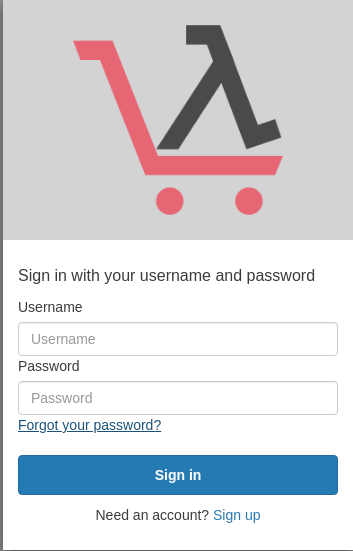
\includegraphics[scale=0.3]{../../../../Images/userManual/singIN.png}
    \centering
\end{figure}
User is redirected to the sign-up page. Here the user has to insert all his information in the form, all data is mandatory, and the sistem doesn't let the user continue unless he provides all information. \begin{figure}[!ht]
    \caption{Sign-in button}
    \vspace{10px}
    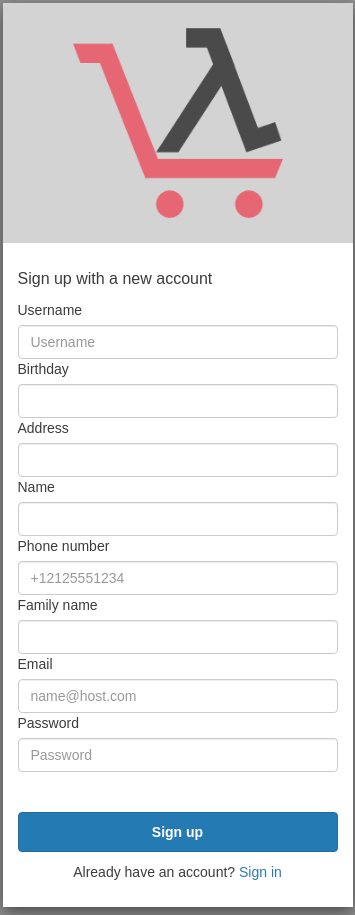
\includegraphics[scale=0.2]{../../../../Images/userManual/signUp.png}
    \centering
\end{figure}The password field must contain a lower case letter, an upper case letter, a special character, a number and has to be at least 8 characters long.
\begin{figure}[!ht]
    \caption{Sign-in button}
    \vspace{10px}
    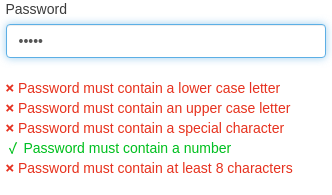
\includegraphics[scale=0.5]{../../../../Images/userManual/insertPWD.png}
    \centering
\end{figure}When the user fills in all the forms correctly he can press the \textit{sign-up} button, and he is redirected to the confermation page that asks a code.
\begin{figure}[!ht]
    \caption{Sign-in button}
    \vspace{10px}
    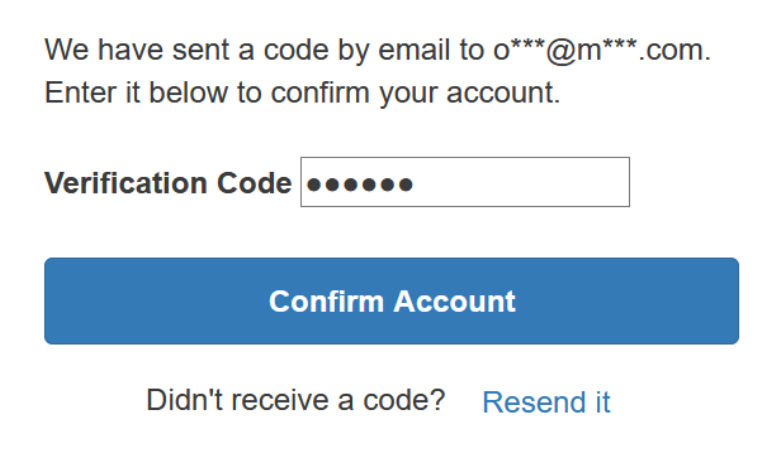
\includegraphics[scale=0.3]{../../../../Images/userManual/confermationCode.png}
    \centering
\end{figure}
The code is sent to the e-mail that the user provided in the previous step. When he recive the e-mail he can insert the code, and he can porced with the registration pressing the \textit{Confirm account} button. Afetr this the user has been successfully registered, and he is redirected to the home page.

\subsubsection{Sign-up error}
If any error happens during the registration procedure such as entering wrong data, you will be redirected to the previous section with an error message describing what the problem is.
\begin{figure}[!ht]
    \caption{Sign-in button}
    \vspace{10px}
    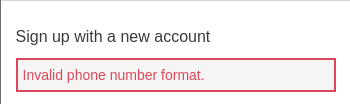
\includegraphics[scale=0.5]{../../../../Images/userManual/wrongData.png}
    \centering
\end{figure}
\subsection{Sign-in}
A user that has previously logged in to the platform can sign-in with his account. To perform this action the user has to click the \textit{sign-in/up} button present in the header.
\begin{figure}[!ht]
    \caption{Sign-in button}
    \vspace{10px}
    
\includegraphics[scale=0.5]{../../../../Images/userManual/signInButton.png}
    \centering
\end{figure}
When the button is pressed the is redirected to sign-in page provided by \textit{Amazon Cognito}. Here he can inset his data:
\begin{itemize}
    \item username;
    \item password.
\end{itemize}
\begin{figure}[!ht]
    \caption{Sign-in form}
    \vspace{10px}
    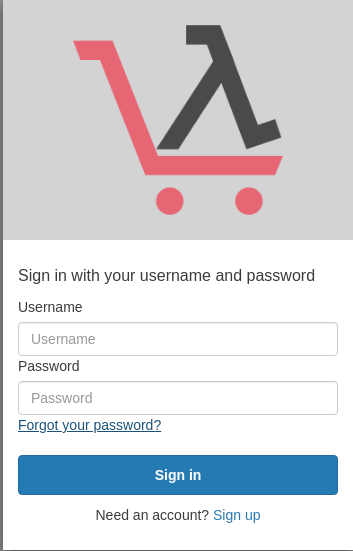
\includegraphics[scale=0.3]{../../../../Images/userManual/singIN.png}
    \centering
\end{figure}
\subsubsection{Login error}
If the user provides wrong credential a message error appeat to inform the user of the error.
\begin{figure}[!ht]
    \caption{Sign-in form}
    \vspace{10px}
    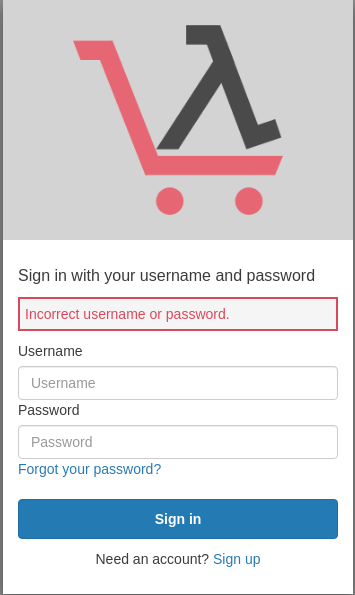
\includegraphics[scale=0.3]{../../../../Images/userManual/singInError.png}
    \centering
\end{figure}
\subsubsection{Forgetten password}
If a user forgot his password he can change it using the appropriate function. To achieve this the user has to open the \textit{forgot your password} link. After this he has to insert his username in the appropriate form.
\begin{figure}[!ht]
    \caption{Forgot password}
    \vspace{10px}
    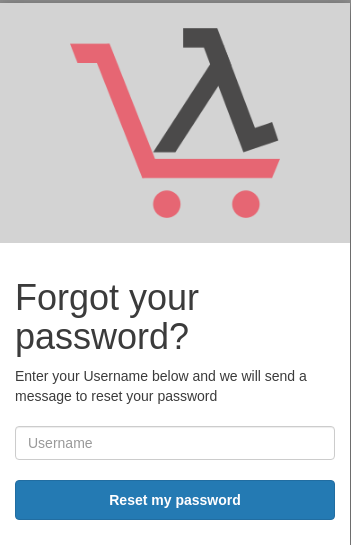
\includegraphics[scale=0.3]{../../../../Images/userManual/forgotPWD.png}
    \centering
\end{figure}
Whern this an e-mail with a verification code is sent to the e-mail used for the registration of the account. With this code the user can change his password using the provided form. When the user preses the confermation button the password is changed.
\begin{figure}[!ht]
    \caption{Change password form}
    \vspace{10px}
    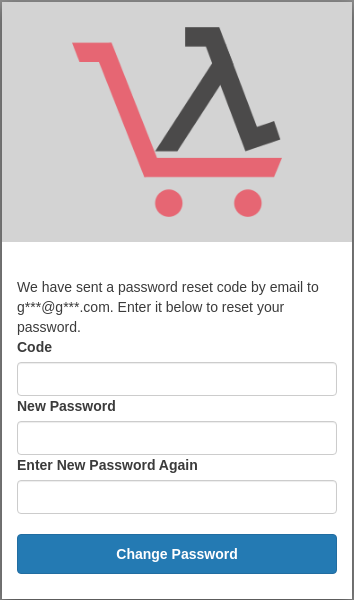
\includegraphics[scale=0.3]{../../../../Images/userManual/changingPWD.png}
    \centering
\end{figure}
\subsection{Browsing products}
A generic user can see the salable products. He can see these products in the Homepage sorted for products on sale and products in low quantity and in the product list page accessible from the \textit{products} button in the header, here the user can see all salable products.
\begin{figure}[!ht]
    \caption{Browsing products}
    \vspace{10px}
    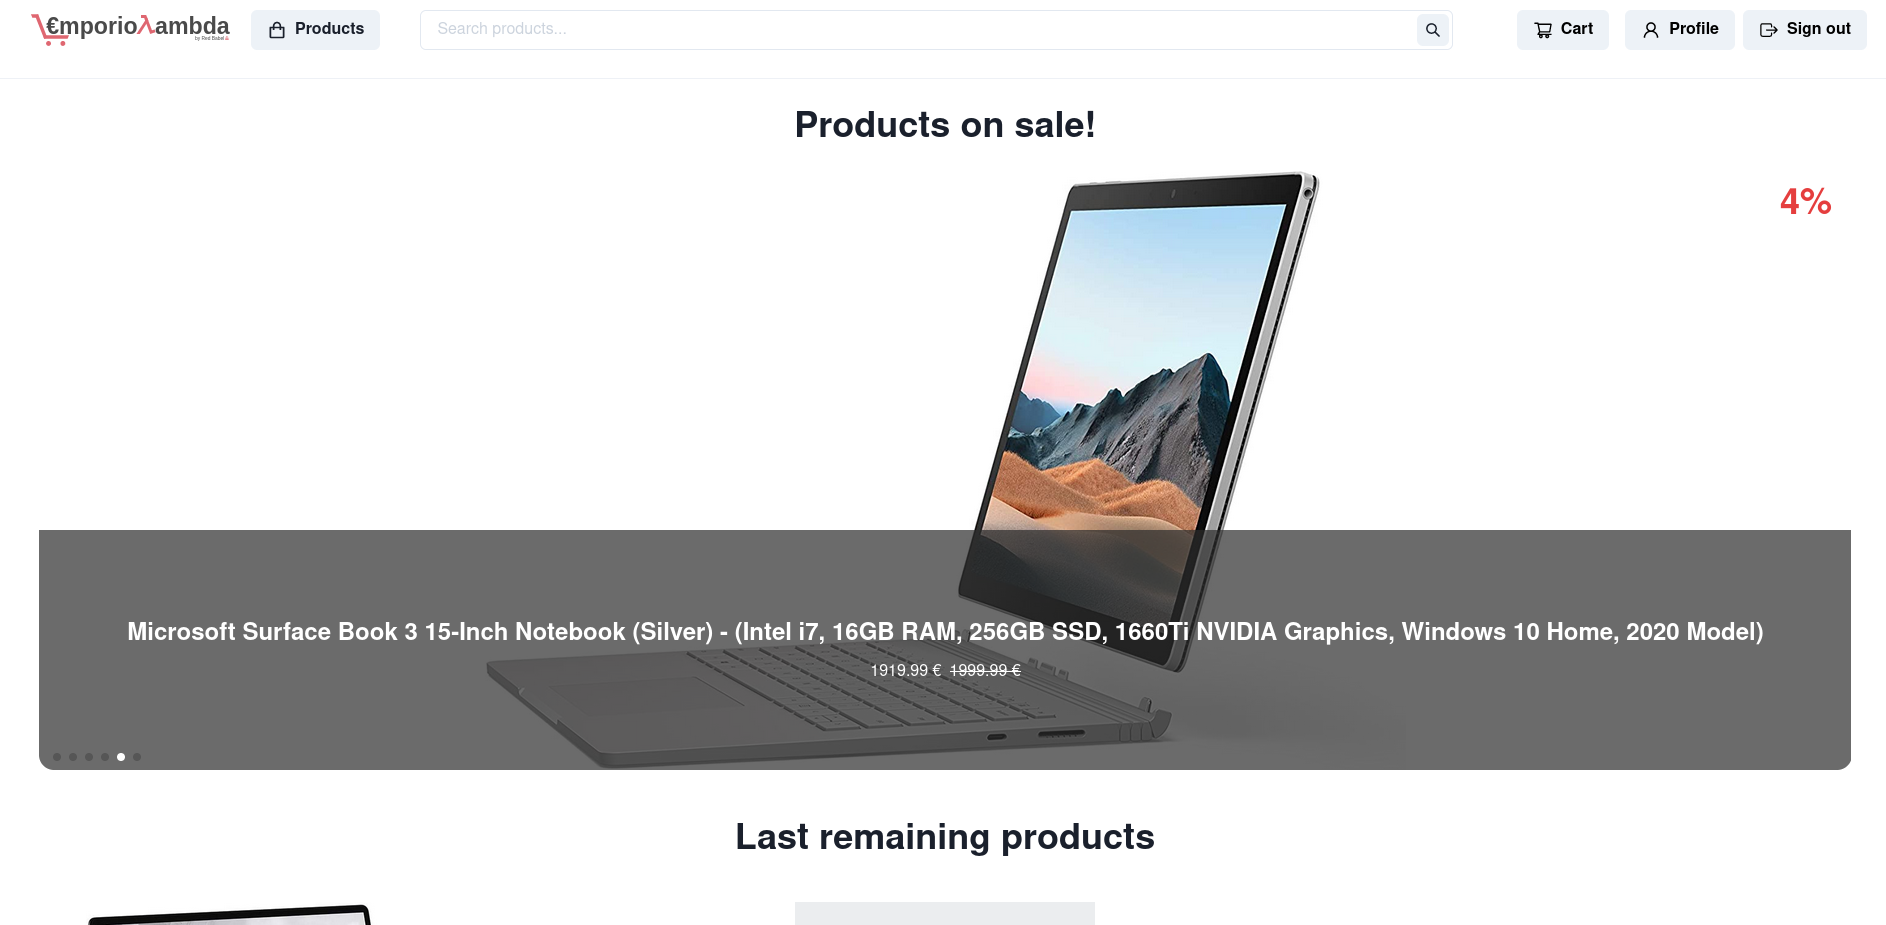
\includegraphics[scale=0.2]{../../../../Images/userManual/home.png}
    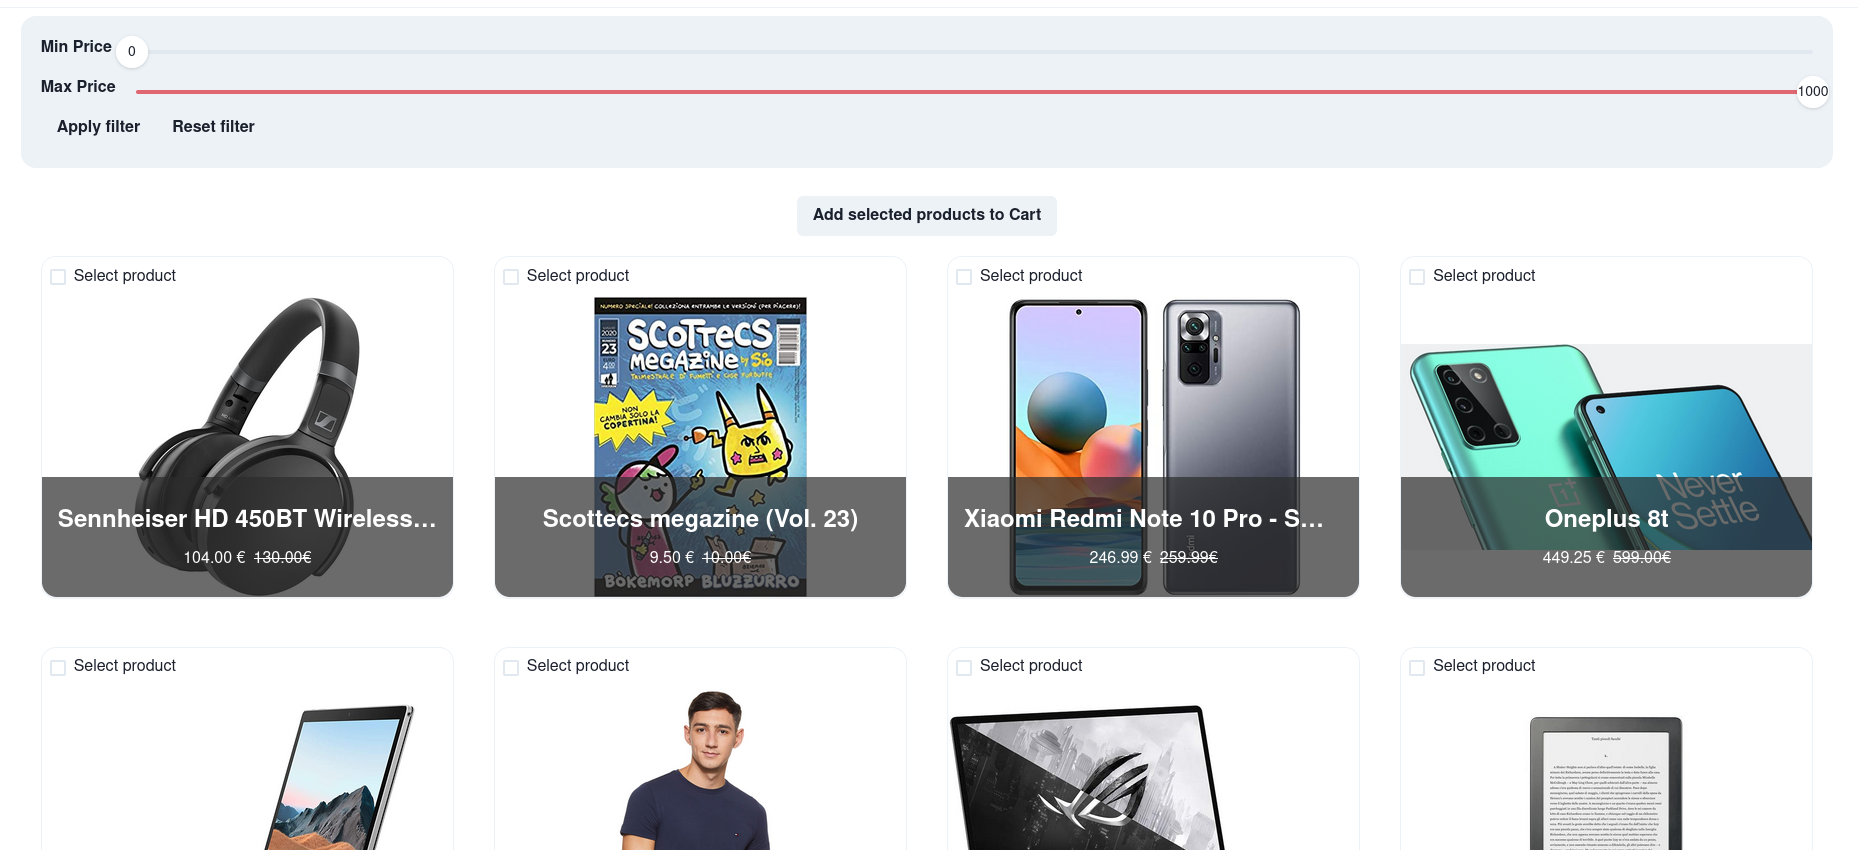
\includegraphics[scale=0.3]{../../../../Images/userManual/PLP.png}

    \centering
\end{figure}

\subsection{Searching and filtering products}
A generic user can search and filter products by price to achieve this he has to:
\begin{itemize}
    \item  \textit{Searching products}: the user can insert a keyword inside the searchbar in the header identifiable by the text \textit{Search products...} and press enter or clicking the search button identifiable by the search lens icon.
          \begin{figure}[!ht]
              \caption{Searching products}
              \vspace{10px}
              
\includegraphics[scale=0.2]{../../../../Images/userManual/searcbar.png}
              \centering
          \end{figure}
    \item \textit{Filtering by price}: the user inside the PLP using the slider on the top of the page can set the range of price with a minimun or maximum price or both, and after click \textit{Apply filter} button.
          \begin{figure}[!ht]
              \caption{Filter for products}
              \vspace{10px}
              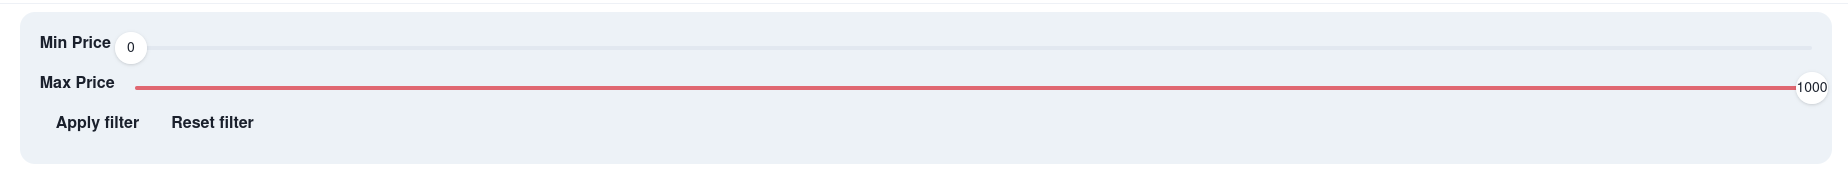
\includegraphics[scale=0.2]{../../../../Images/userManual/filter.png}
              \centering
          \end{figure}
\end{itemize}
\subsection{Viewing product detail}
To see the product detail a user has to press the product image, both in the home and in the PLP.
\begin{figure}[!ht]
    \caption{Product detail page}
    \vspace{10px}
    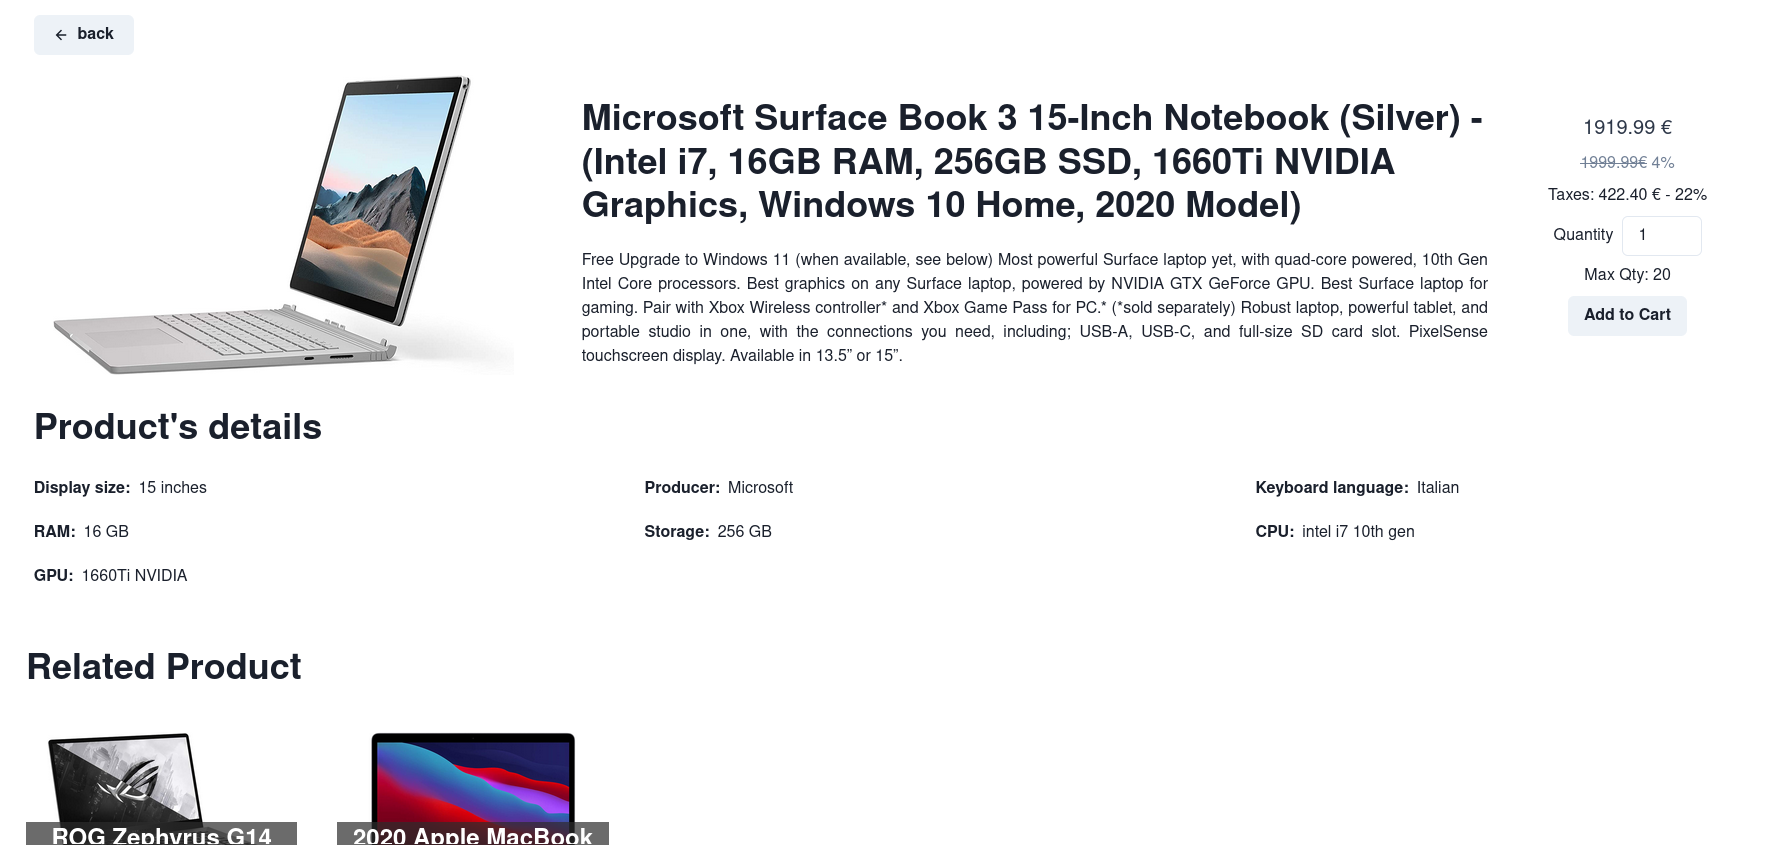
\includegraphics[scale=0.2]{../../../../Images/userManual/PDP.png}
    \centering
\end{figure}
He is redirected to the product detail page where he can see:
\begin{itemize}
    \item the product's title;
    \item the product's image;
    \item the product's description;
    \item the product's details;
    \item the product's price with the discounted price with the discount percentage if any ;
    \item the product's taxes;
    \item the product's availability;
    \item alternative produts.
\end{itemize}
\subsection{Adding products to the cart}
The user has two options to add products to the cart.
\begin{itemize}
    \item \textit{Directly from the product list page:} by seleting the products that he wants to add cart cheekcing the checkbox present in each of the product images, and clicking the \textit{add selected products to cart} button. In this way the user can add multiple porducts to the cart.
          \begin{figure}[!ht]
              \caption{Adding to cart multiple products}
              \vspace{10px}
              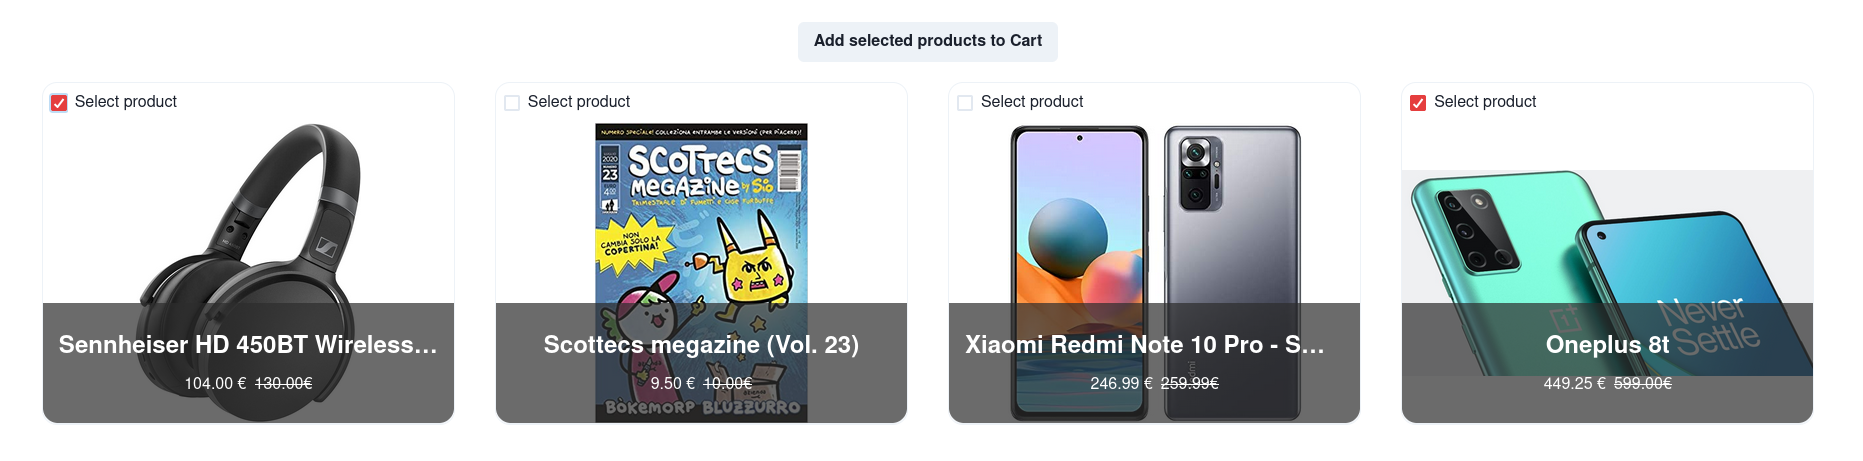
\includegraphics[scale=0.25]{../../../../Images/userManual/addtoCartPLP.png}
              \centering
          \end{figure}
    \item \textit{Form product's detail page:} When the user is in the detail page of a product he can add that product to the cart pressing the \textit{add to cart button} he can also set the quantity of products he wants to add to the cart.
          \begin{figure}[!ht]
              \caption{Adding to cart a product}
              \vspace{10px}
              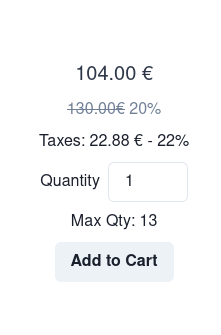
\includegraphics[scale=0.5]{../../../../Images/userManual/addToCartPDP.png}
              \centering
          \end{figure}
\end{itemize}
When the button is pressed a pop-up showing two buttons appears. One to continue to the cart and the other to return to the PLP page.
\begin{figure}[!ht]
    \caption{Add to cart result popup}
    \vspace{10px}
    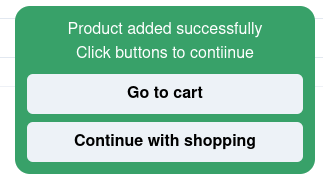
\includegraphics[scale=0.5]{../../../../Images/userManual/cartResult.png}
    \centering
\end{figure}
\subsection{Managing the cart}
A user can access the cart when he adds a product to the cart or by clicking the \textit{cart} button presnt in the header.
\begin{figure}[!ht]
    \caption{Cart page}
    \vspace{10px}
    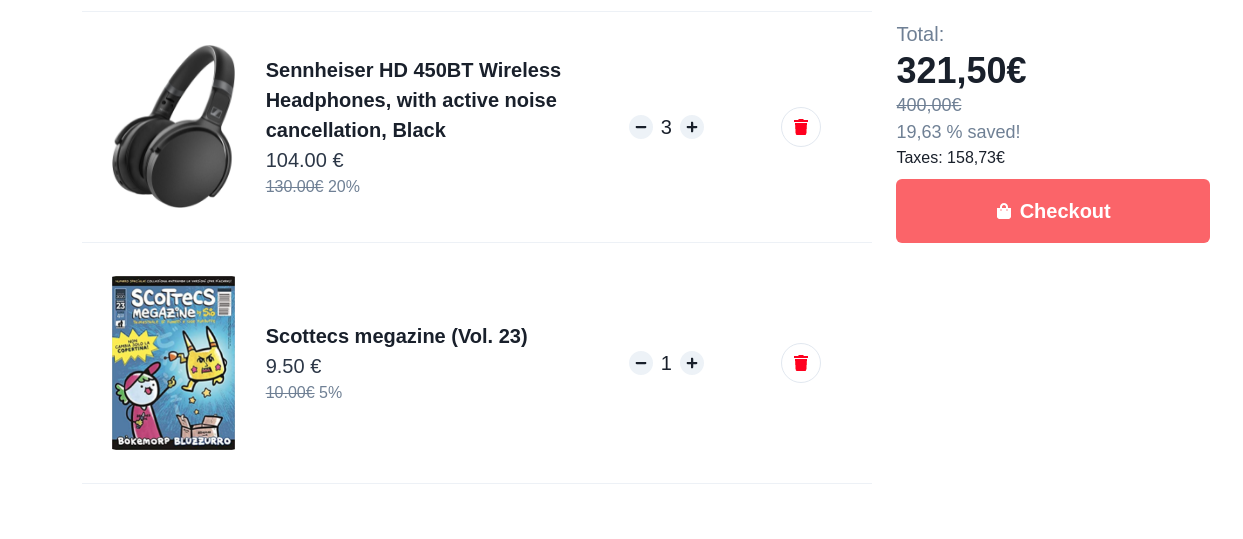
\includegraphics[scale=0.3]{../../../../Images/userManual/cart.png}
    \centering
\end{figure}
In the cart the user can see all the products that he previusly add to the cart. For each product he can see:
\begin{itemize}
    \item the product's title;
    \item the product's image;
    \item the product's description;
    \item the product's price and the discounted price with the discount percentage if any ;
    \item the product's quantity.
\end{itemize}
He can also manage the quantity by clicking the less or more buttons, to delete a product the user has to click the trash button. In the right part of the cart there is the cart summary where the user can see:
\begin{itemize}
    \item the cart's total price and the discounted price with the discount percentage if any ;
    \item the taxes of the entire cart.
\end{itemize}


\section{Customer instructions}
\subsection{Signing out}
An authenticated user can sign out from the platform. To perform this action the user needs to click the sign-out button that is present in the header. When the button is pressed user is logged out form platform.
\begin{figure}[!ht]
    \caption{Header}
    \vspace{10px}
    
\includegraphics[scale=0.25]{../../../../Images/userManual/signOut.jpg}
    \centering
\end{figure}
\subsection{Viewing and editing user data}
An authenticated user can view and modify his data.
\subsubsection{Viewing user data}
To perform this action the authenticated user has to click the profile button.
\begin{figure}[!ht]
    \caption{Button detail}
    \vspace{10px}
    
\includegraphics[scale=0.5]{../../../../Images/userManual/profile-signoutButton.png}
    \centering
\end{figure}
When the button is pressed the user see the dashbord page, were all his data is shown.
\begin{figure}[!ht]
    \caption{User data}
    \vspace{10px}
    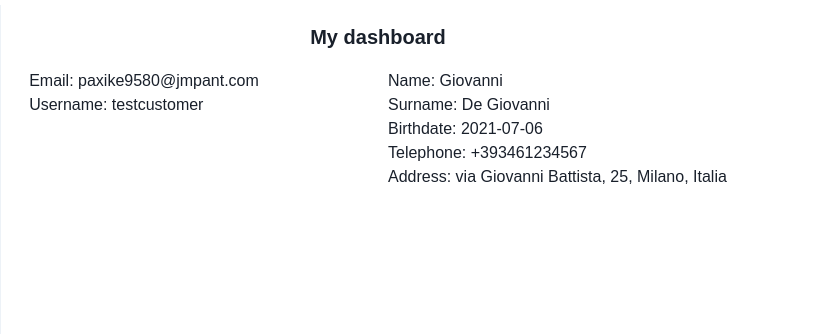
\includegraphics[scale=0.5]{../../../../Images/userManual/profileDshboard.png}
    \centering
\end{figure}
\newpage
\subsubsection{Modify user data}
When user is in the profile page he can press the \textit{Edit profile} button present in the profile navbar.
\begin{figure}[!ht]
    \caption{Profile page navbar}
    \vspace{10px}
    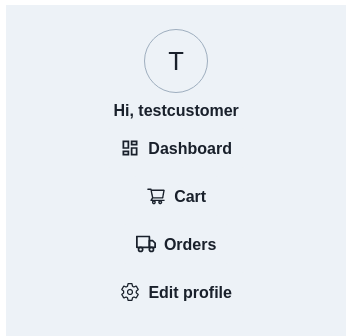
\includegraphics[scale=0.5]{../../../../Images/userManual/dashboardNavBar.png}
    \centering
\end{figure}
When the button is pressed the user see the page for modify his data. He can change the data that he wants to modify using the proper form.
\begin{figure}[!ht]
    \caption{Profile page navbar}
    \vspace{10px}
    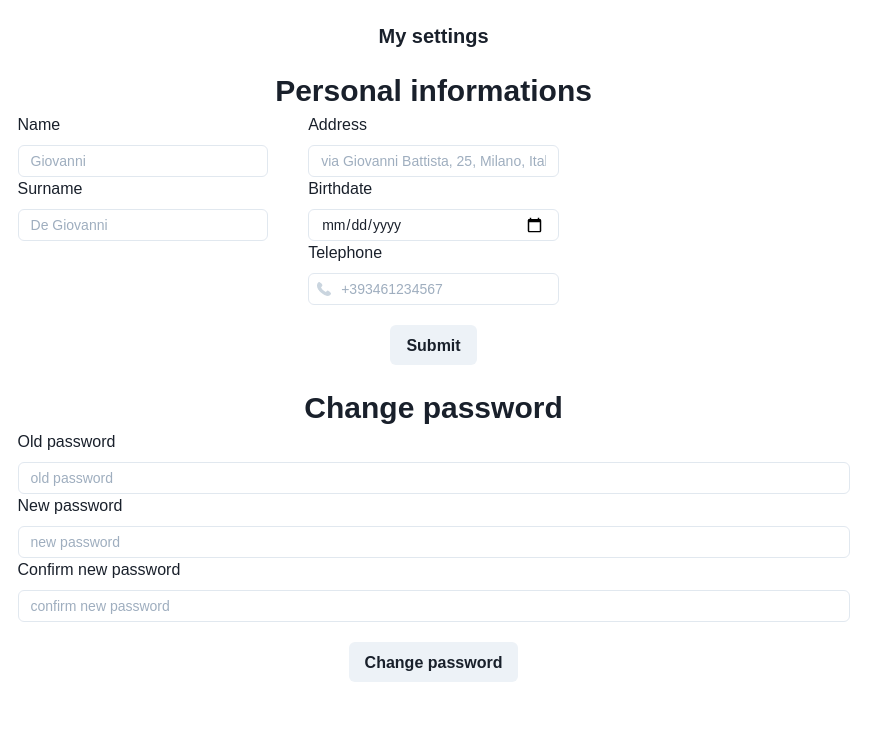
\includegraphics[scale=0.3]{../../../../Images/userManual/profileModfication.png}
    \centering
\end{figure}
\\
When he clicks the submit button a pop-up appears to indicate the result of the action. With the popup the user can return to the profile dashboard.
\newpage
\subsection{Check out}
An authenticated user can perform the checkout. To perform this action the user must be logged, and he has to be in the cart page.
\begin{figure}[!ht]
    \caption{Cart page}
    \vspace{10px}
    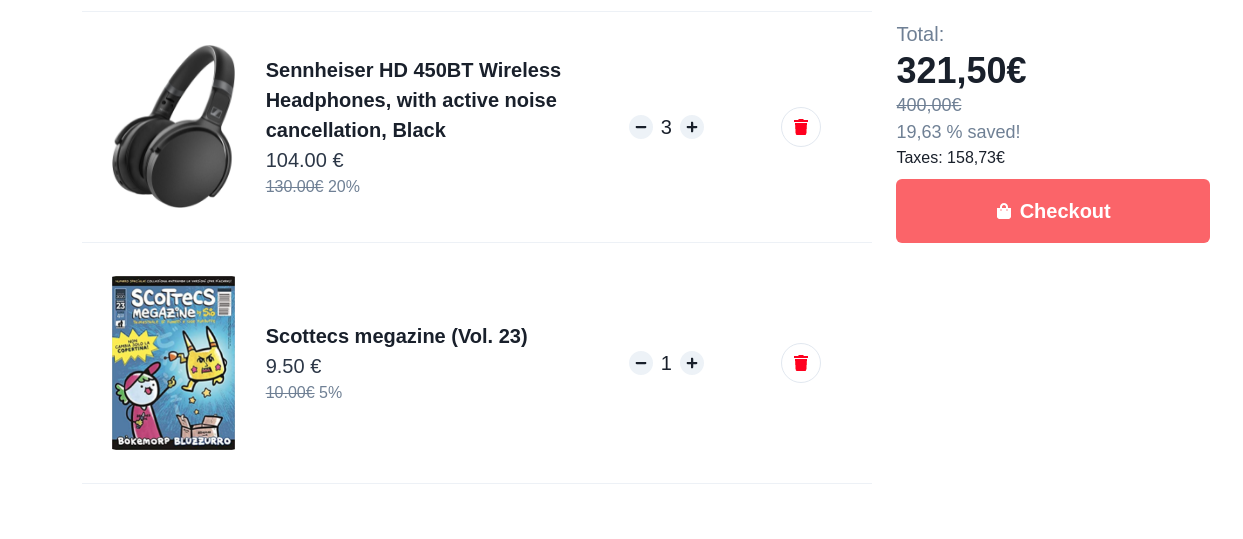
\includegraphics[scale=0.35]{../../../../Images/userManual/cart.png}
    \centering
\end{figure}
\\
He can press the checkout button that redirect him to the stripe checkout.
\begin{figure}[!ht]
    \caption{Checkout}
    \vspace{10px}
    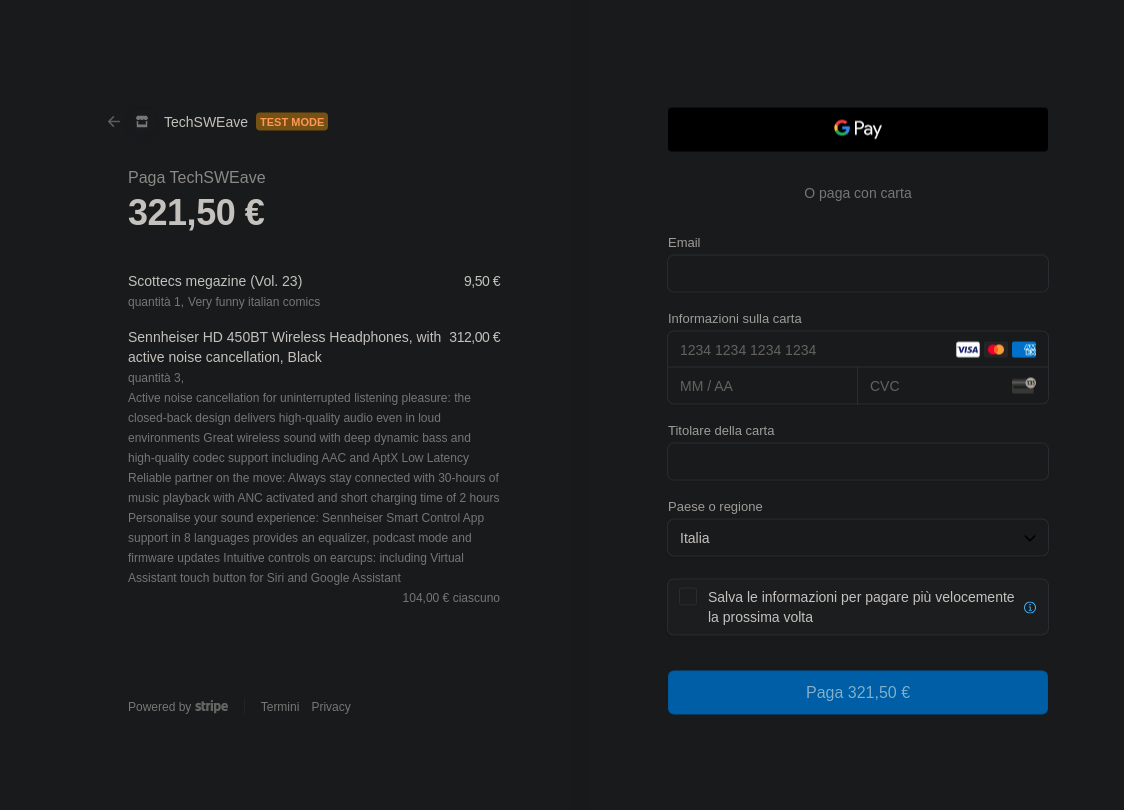
\includegraphics[scale=0.3]{../../../../Images/userManual/checkout.png}
    \centering
\end{figure}
\\
The user now has to insert:
\begin{itemize}
    \item e-mail;
    \item card number;
    \item expiration date:
    \item cvc;
    \item name.
\end{itemize}
The user can also use other payment method like \textit{Gpay} and \textit{Apple Pay}.
When the user entred all the required information he can click the checkout payment button to pay the order. After this he is redirected to the succes page and here he can go to his order page list, or if the checkout fail to the cart page.
\begin{figure}[!ht]
    \caption{Checkout success}
    \vspace{10px}
    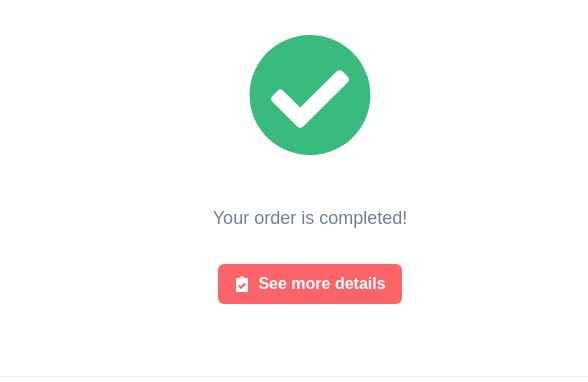
\includegraphics[scale=0.5]{../../../../Images/userManual/checkoutSuccess.png}
    \centering
\end{figure}
\subsection{Order list visualization}
An authenticated user can view all his previus order. To perform this action the user has to be in the profile page, and he has to click the \textit{order} button.
\begin{figure}[!ht]
    \caption{Profile page navbar}
    \vspace{10px}
    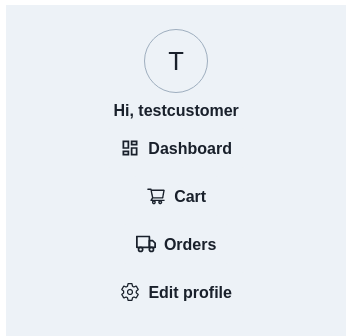
\includegraphics[scale=0.5]{../../../../Images/userManual/dashboardNavBar.png}
    \centering
\end{figure}
\newpage
When the button is pressed the order list is shown. There is two differnt view for order list depending on the device in use.
\begin{itemize}
    \item Desktop visualization:
          the user see all his order with produt information like:
          \begin{figure}[!ht]
              \caption{Desktop order}
              \vspace{10px}
              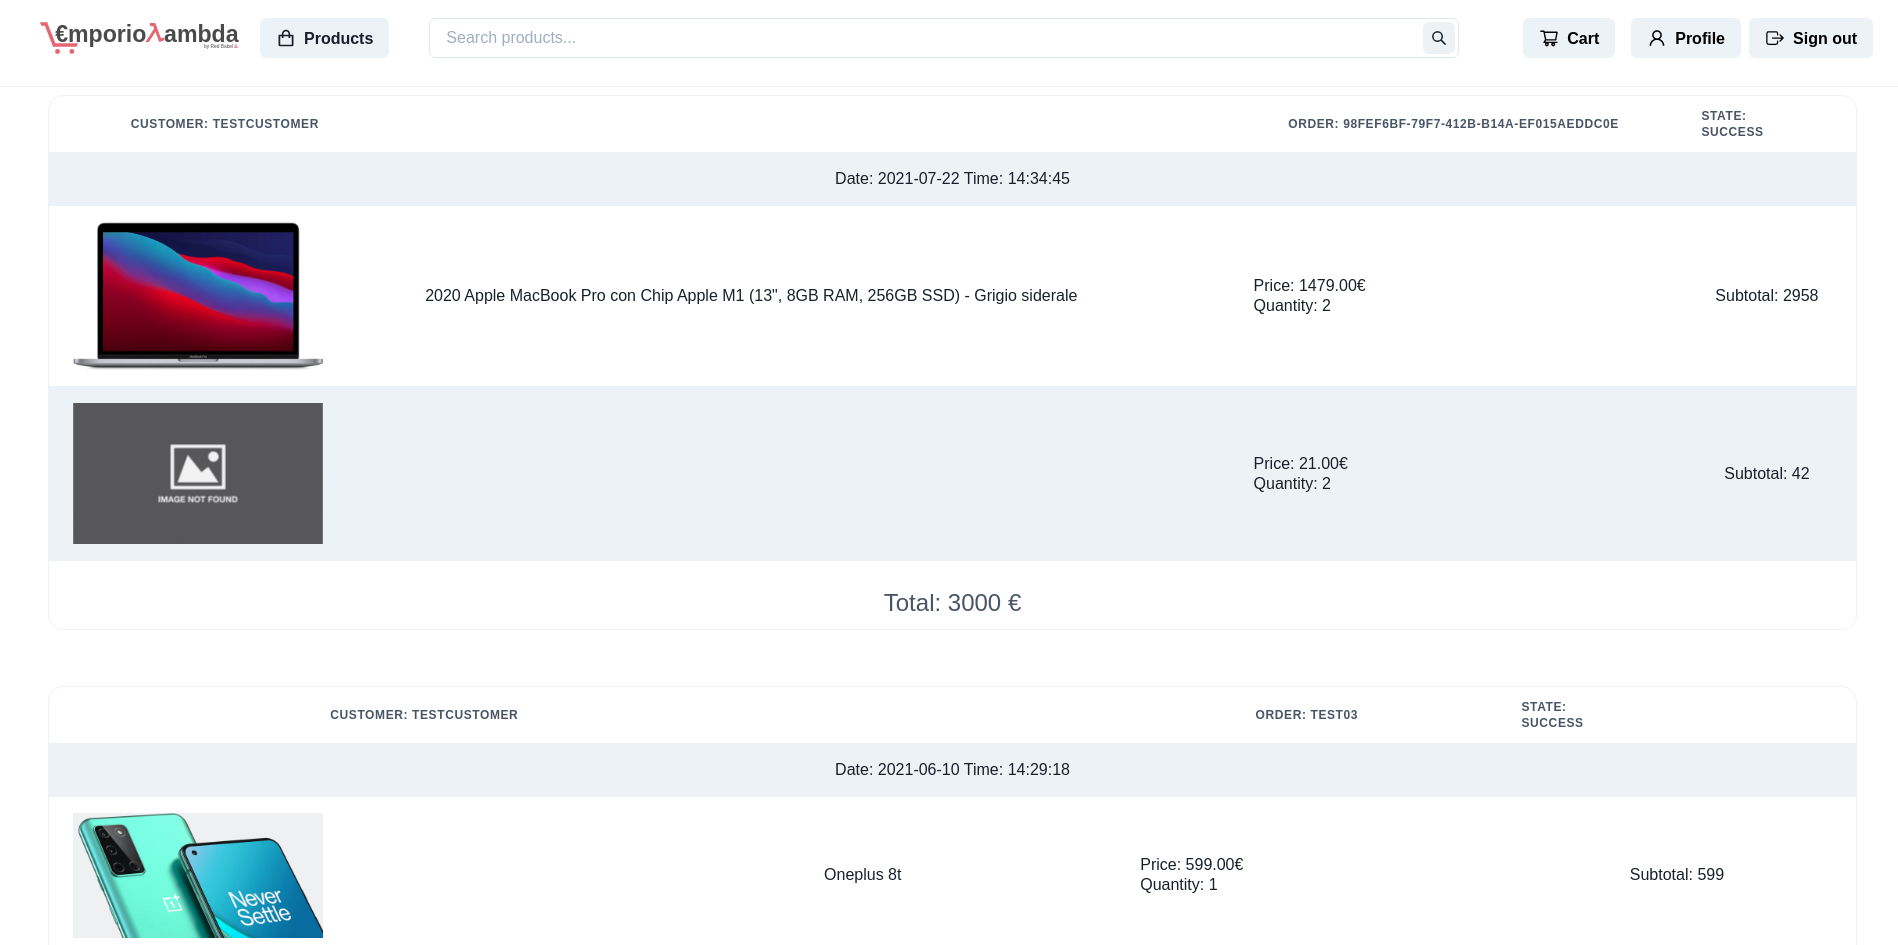
\includegraphics[scale=0.2]{../../../../Images/userManual/orderDesktop.png}
              \centering
          \end{figure}
          \\
          \begin{itemize}
              \item username;
              \item order ID;
              \item order date;
              \item title;
              \item image;
              \item price;
              \item qunatity;
              \item description;
              \item order state;
              \item total of the single product;
              \item total of the order;
          \end{itemize}
          \newpage
    \item Mobile visualization
          \begin{figure}[!ht]
              \caption{Mobile order}
              \vspace{10px}
              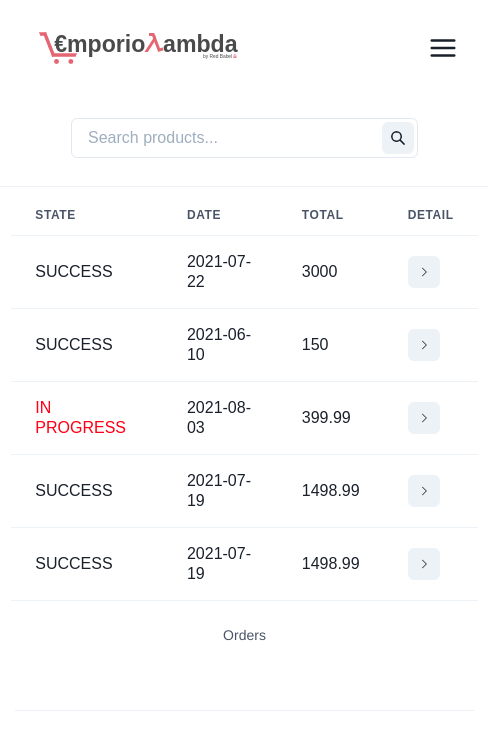
\includegraphics[scale=0.3]{../../../../Images/userManual/orderMobile.png}
              \centering
          \end{figure}
          the user see an order list with:
          \begin{itemize}
              \item order state;
              \item order date;
              \item total;
              \item detail butto.
          \end{itemize}
          When the user from mobile clicks the detial button he is redirected to the order detail where he can see all the order information like desktop visualization.
          \begin{figure}[!ht]
              \caption{Mobile order detail}
              \vspace{10px}
              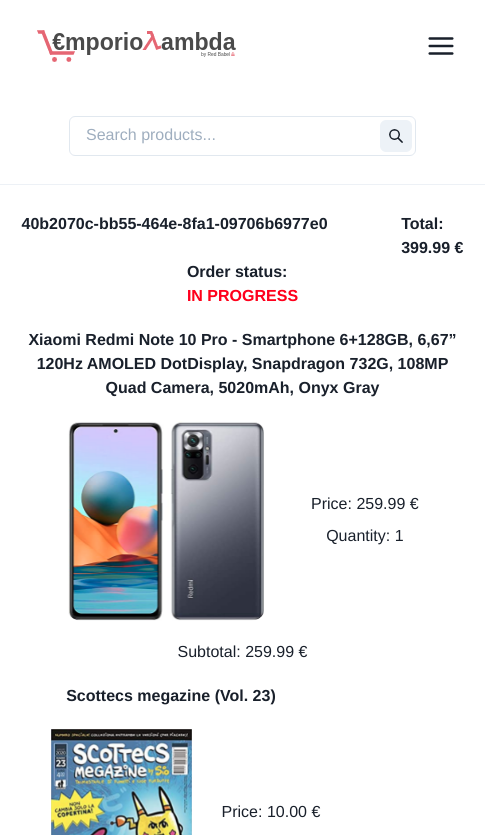
\includegraphics[scale=0.2]{../../../../Images/userManual/oderMobileDetail.png}
              \centering
          \end{figure}

\end{itemize}

\section{Vendor instructions}
\subsection{Orders view}
By clicking on the \textit{Orders} button in the header, the vendor reaches the orders page, where he can view all the orders placed by customers.
\newline
From this page the vendor can view for each order:
\begin{itemize}
    \item the order code;
    \item the status of the order;
    \item the total and subtotal price;
    \item the quantity of ordered items;
    \item the checkout date;
    \item the username of the customer who placed the order.
\end{itemize}
\begin{figure}[!ht]
    \caption{Orders page viewed from the vendor}
    \vspace{5px}
    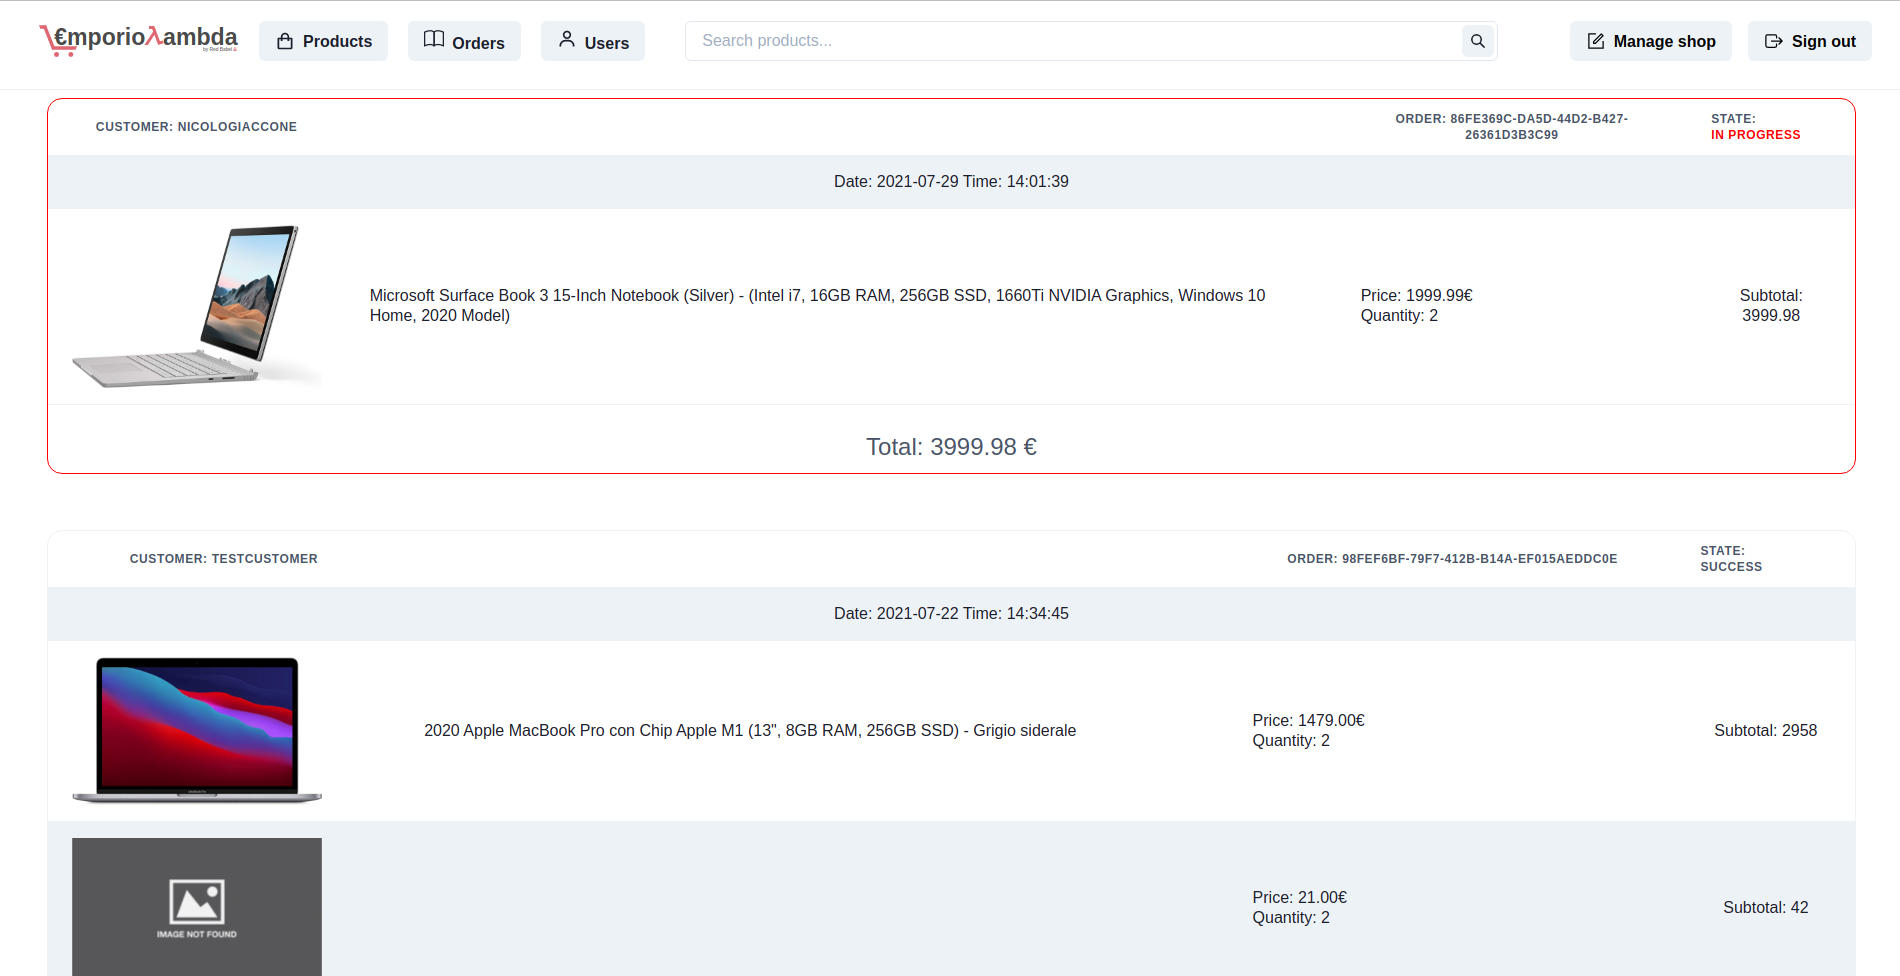
\includegraphics[scale=0.25]{../../../../Images/userManual/ordersVendor.png}
    \centering
\end{figure}
\pagebreak
\subsection{Shop management}
By clicking on the \textit{Manage shop} button in the header, the vendor reaches the page to manage the shop, where he can create a new product, create a new category or delete a category.
\subsubsection{Create new product}
By clicking on \textit{Create New Product}, a screen will be displayed where the vendor can insert a new product in the system. Here the vendor can:
\begin{itemize}
    \item enter the product title;
    \item enter the price of the product;
    \item enter the description;
    \item enter the discount;
    \item enter the availability;
    \item insert an image of the product;
    \item select the product category;
    \item add notes.
\end{itemize}
Product's title, price, image, availability and category are mandatory, if the vendor doesn't fill that a pop-up error appers and the creation is blocked.
After having entered the necessary data for the new product, it will be possible to insert the product by clicking on the \textit{Submit} button at the bottom of the page.
\begin{figure}[!ht]
    \caption{Create new product section viewed from the vendor}
    \vspace{5px}
    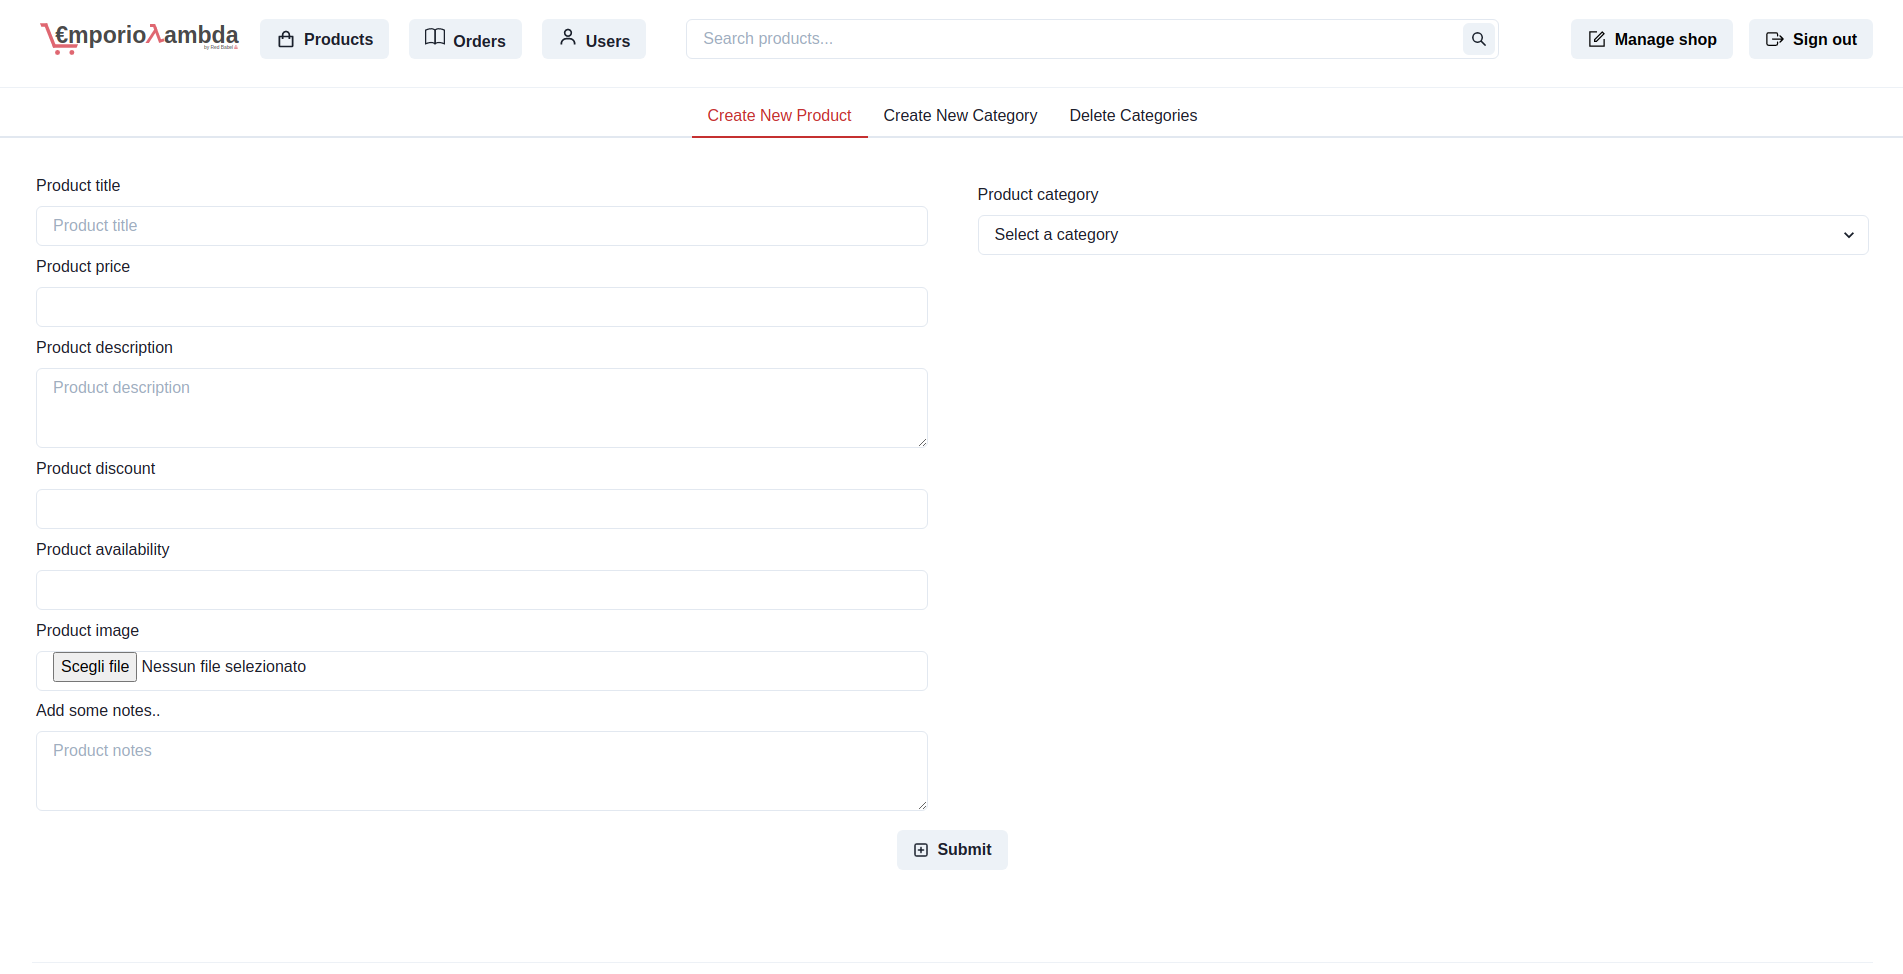
\includegraphics[scale=0.25]{../../../../Images/userManual/createNewProductVendor.png}
    \centering
\end{figure}
\pagebreak
\subsubsection{Create new category}
By clicking on \textit{Create New Category}, a screen will be displayed where the vendor can insert a new category of products in the system. Here the vendor can:
\begin{itemize}
    \item enter the category name;
    \item enter the description;
    \item enter the taxation for the category;
    \item add additional customizable specifications based on the category.
\end{itemize}
After entering the necessary data for the new category, it will be possible to insert the category by clicking on the \textit{Submit} button at the bottom of the page.
\begin{figure}[!ht]
    \caption{Create new category section viewed from the vendor}
    \vspace{5px}
    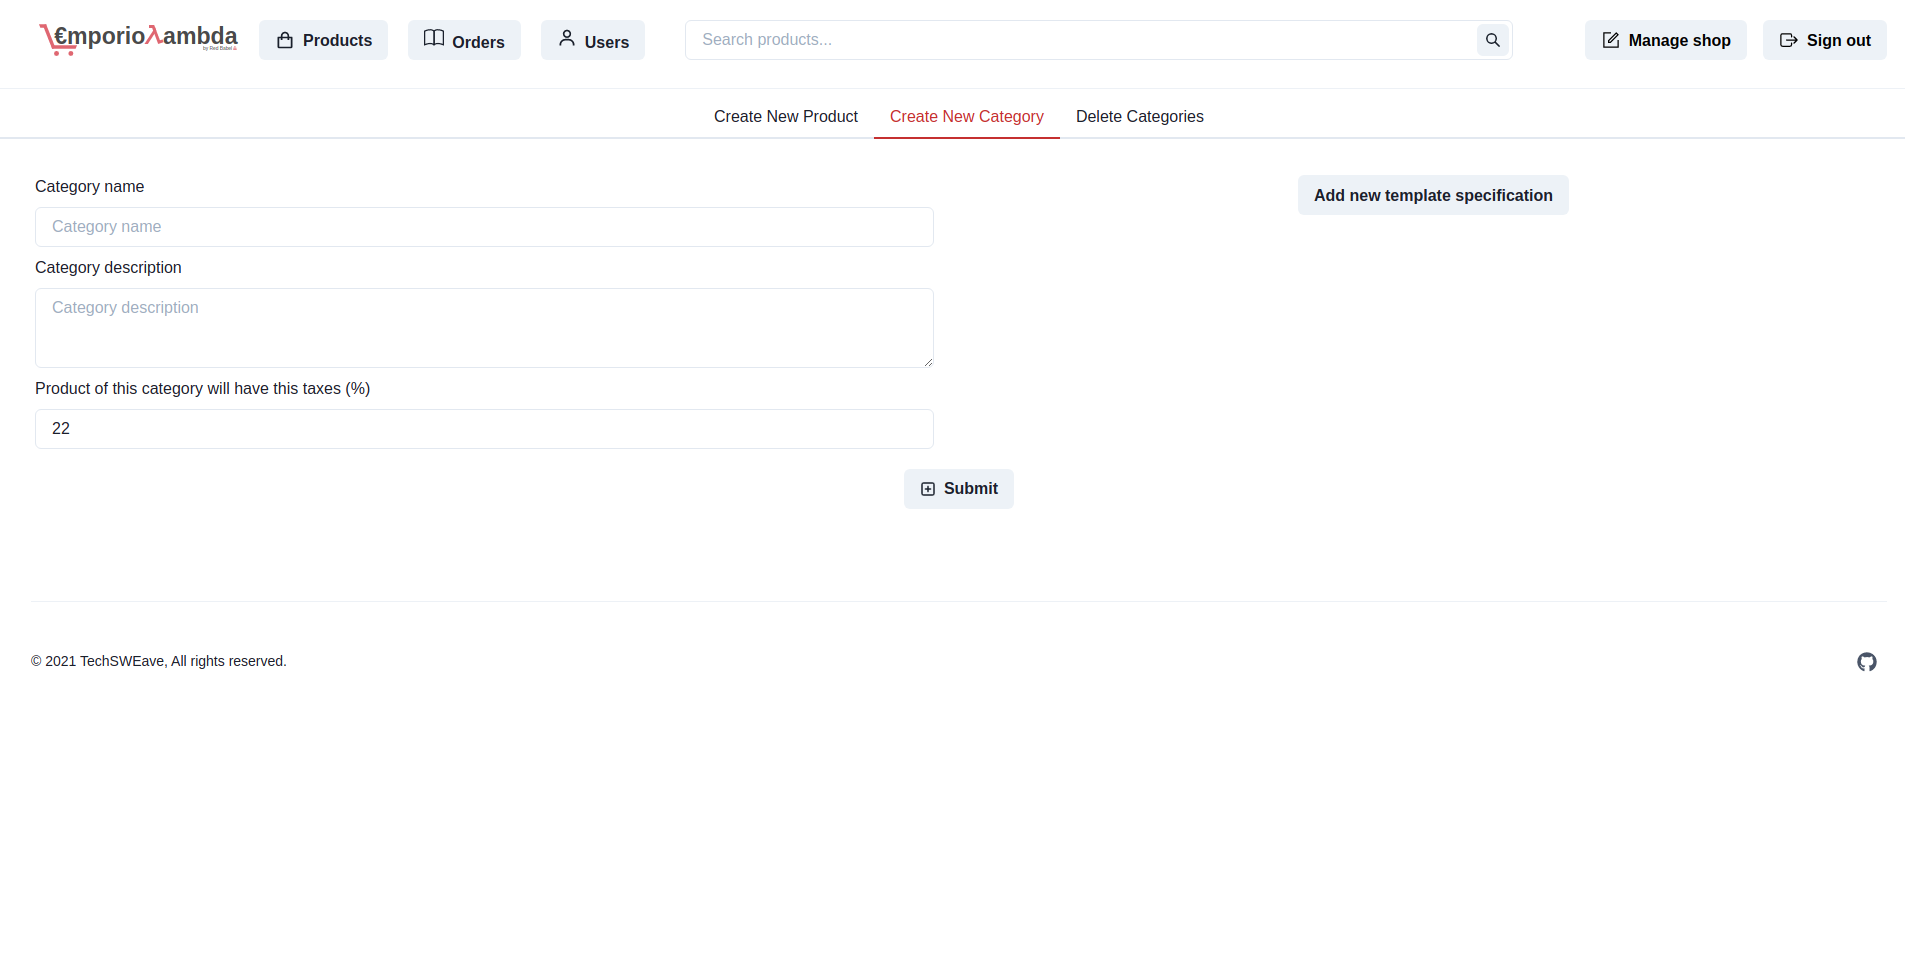
\includegraphics[scale=0.25]{../../../../Images/userManual/createNewCategoryVendor.png}
    \centering
\end{figure}
\subsubsubsection{Add new template specification}
By clicking on the \textit{Add New Template Specification} button displayed at the top right of the screen for adding a new category, the vendor can add one or more additional customizable specifications related to the category.
\linebreak
A row will be displayed for each new specification, in which the vendor can enter:
\begin{itemize}
    \item the name of the specification;
    \item the unit of measurement of the specification.
\end{itemize}
The specifications will finally be added to the category by clicking on the \textit{Submit} button to create the category itself.
\begin{figure}[!ht]
    \caption{Create new category section viewed from the vendor}
    \vspace{5px}
    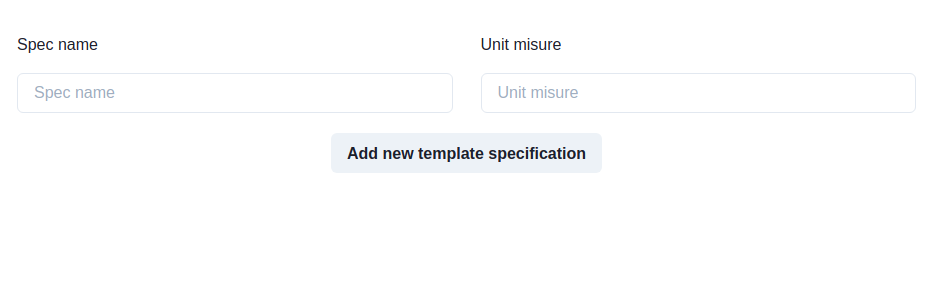
\includegraphics[scale=0.25]{../../../../Images/userManual/addSpecificationCategoryVendor.png}
    \centering
\end{figure}
\pagebreak
\subsubsection{Delete categories}
By clicking on \textit{Delete Categories}, a screen will be displayed where the vendor can delete the categories.\linebreak
To remove a specific category the vendor will have to click on the button \textit{DELETE CATEGORY}, displayed on the bottom of the category that he wants to delete.
\begin{figure}[!ht]
    \caption{Delete categories section viewed from the vendor}
    \vspace{5px}
    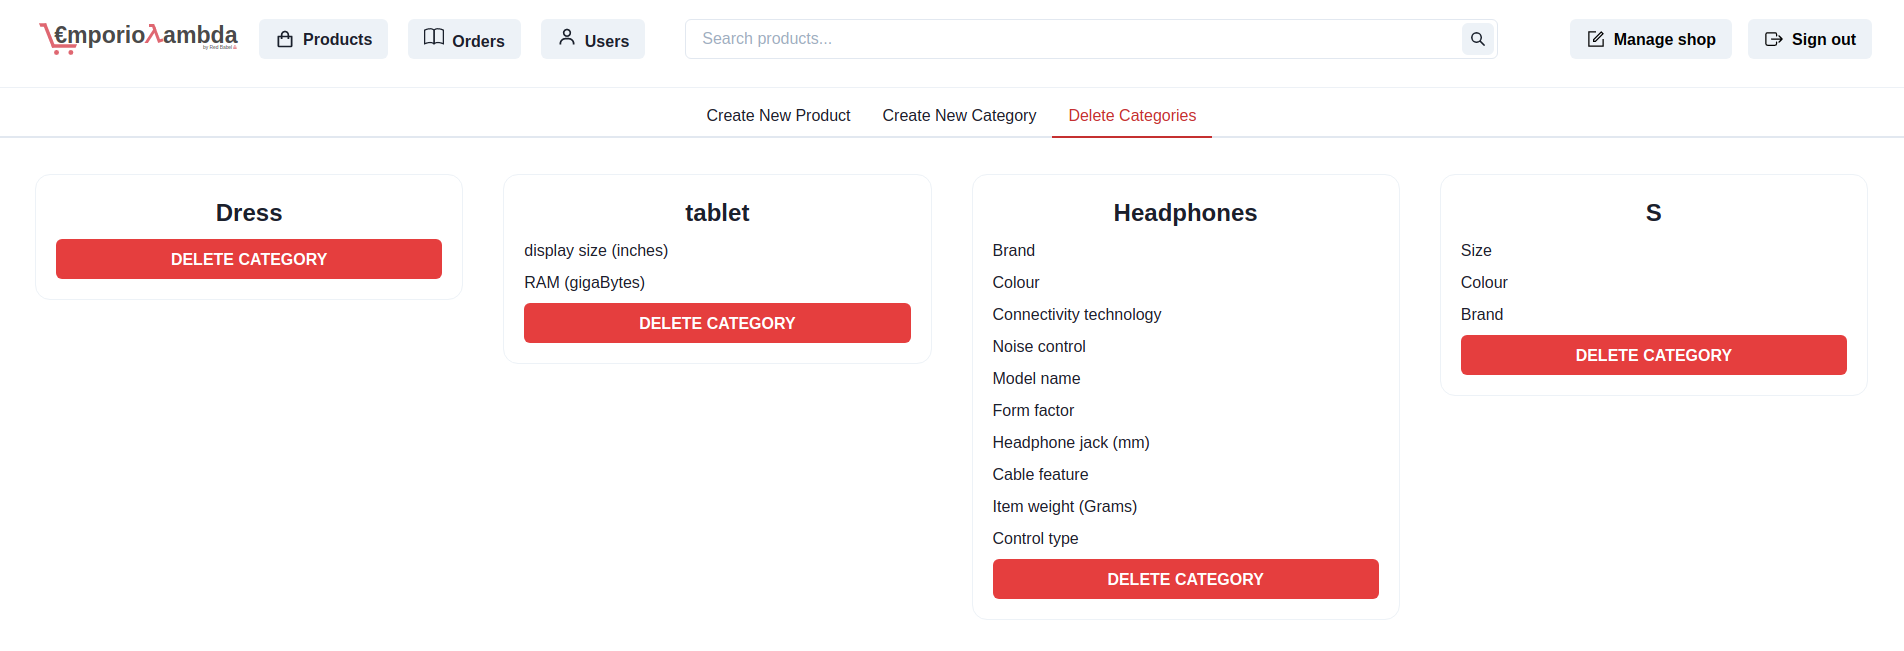
\includegraphics[scale=0.25]{../../../../Images/userManual/deleteCategoriesVendor.png}
    \centering
\end{figure}
\pagebreak
\subsection{Users view}
By clicking on the \textit{Users} button in the header, the vendor reaches the screen to view all registered users on the site.
Here the vendor can view for each user:
\begin{itemize}
    \item the username;
    \item name and surname;
    \item the date of birth;
    \item the address.
\end{itemize}
The vendor can also send an email to the user by clicking directly on the email of the user.
\begin{figure}[!ht]
    \caption{Users page viewed from the vendor}
    \vspace{5px}
    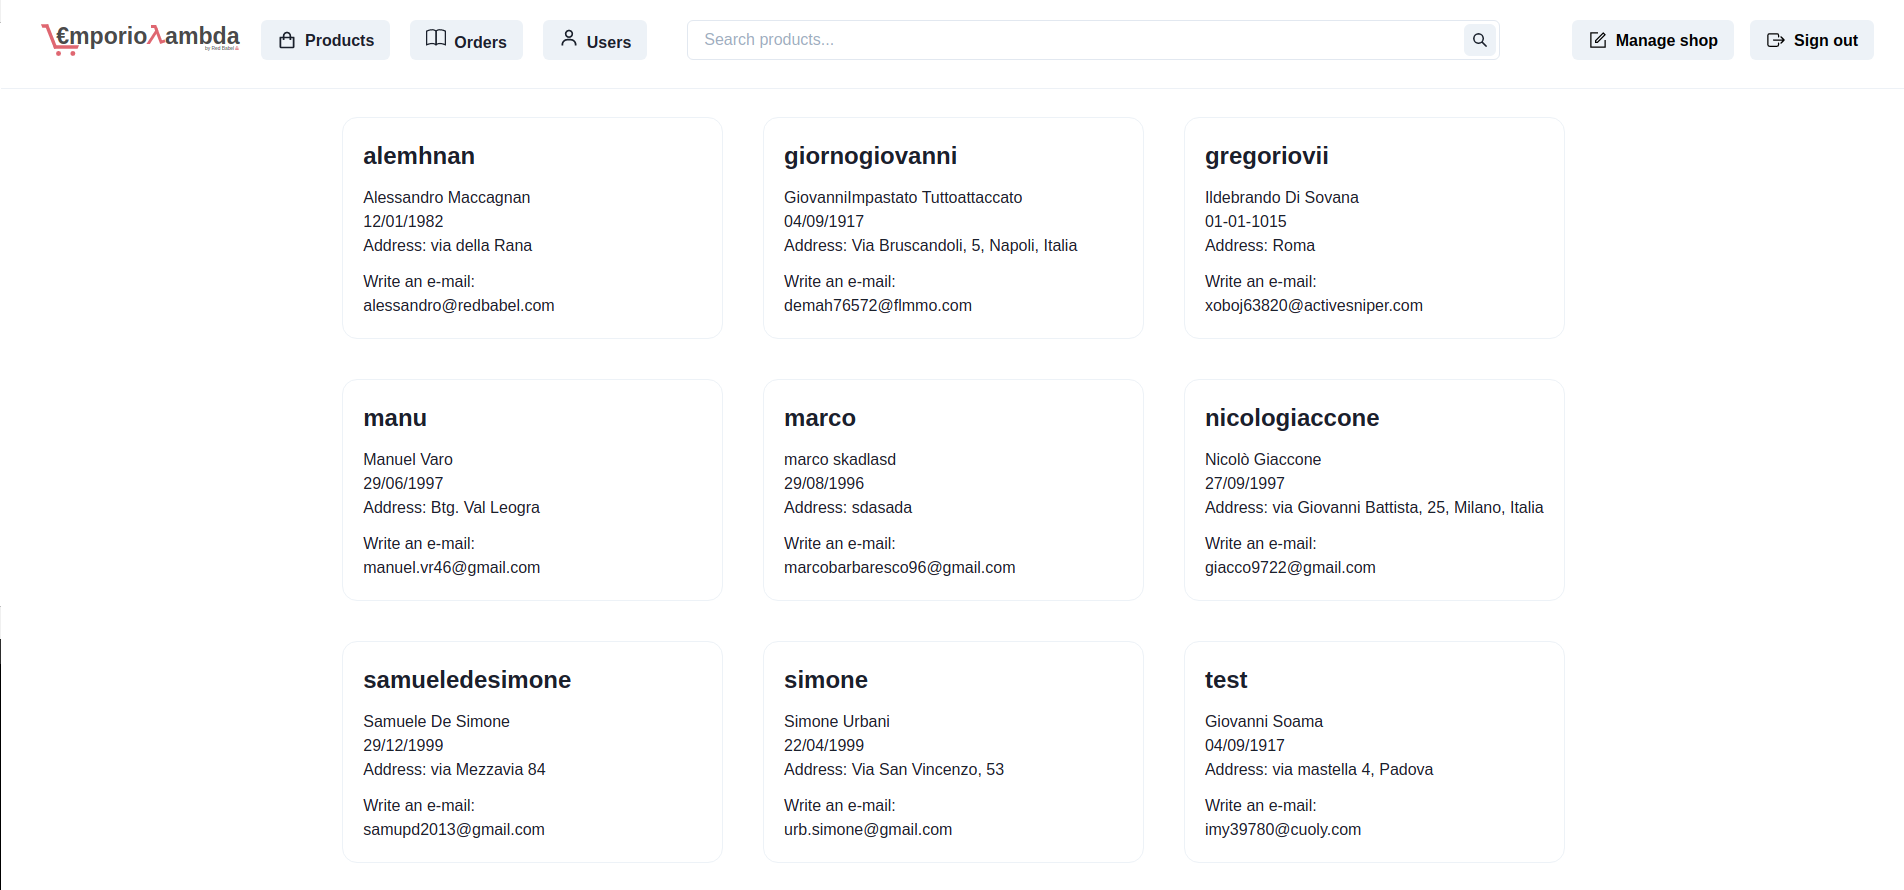
\includegraphics[scale=0.25]{../../../../Images/userManual/usersVendor.png}
    \centering
\end{figure}
\pagebreak
\subsection{Products view}
By clicking on the \textit{Products} button displayed in the top left of the header, the vendor will reach the page from which he can view a list of all the products for sale on the site, both salable and private.
Here the vendor can view for each product:
\begin{itemize}
    \item the image;
    \item the price;
    \item the name.
\end{itemize}
\begin{figure}[!ht]
    \caption{Products page viewed from the vendor}
    \vspace{5px}
    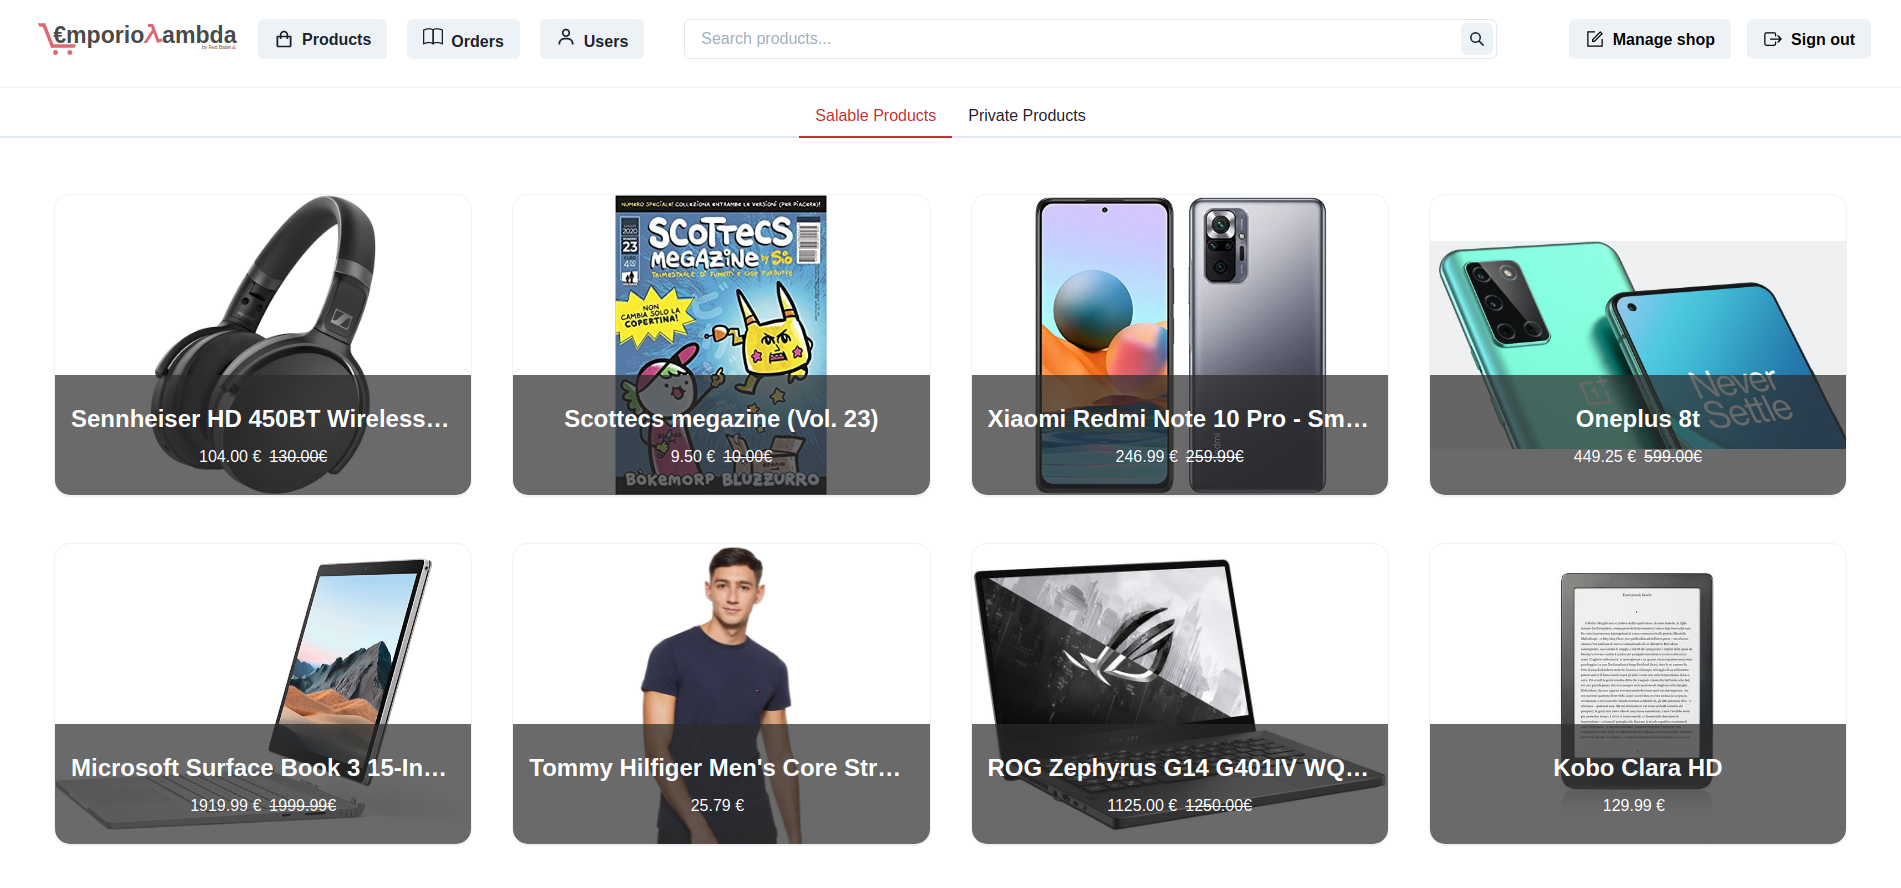
\includegraphics[scale=0.25]{../../../../Images/userManual/productsVendor.png}
    \centering
\end{figure}
\pagebreak
\subsubsection{Product detail}
By clicking on the image of a single product in the products page, the vendor will be redirected to the product detail page, where it will be possible to view all the characteristics of the product and its details.
\begin{figure}[!ht]
    \caption{Product detail page viewed from the vendor}
    \vspace{5px}
    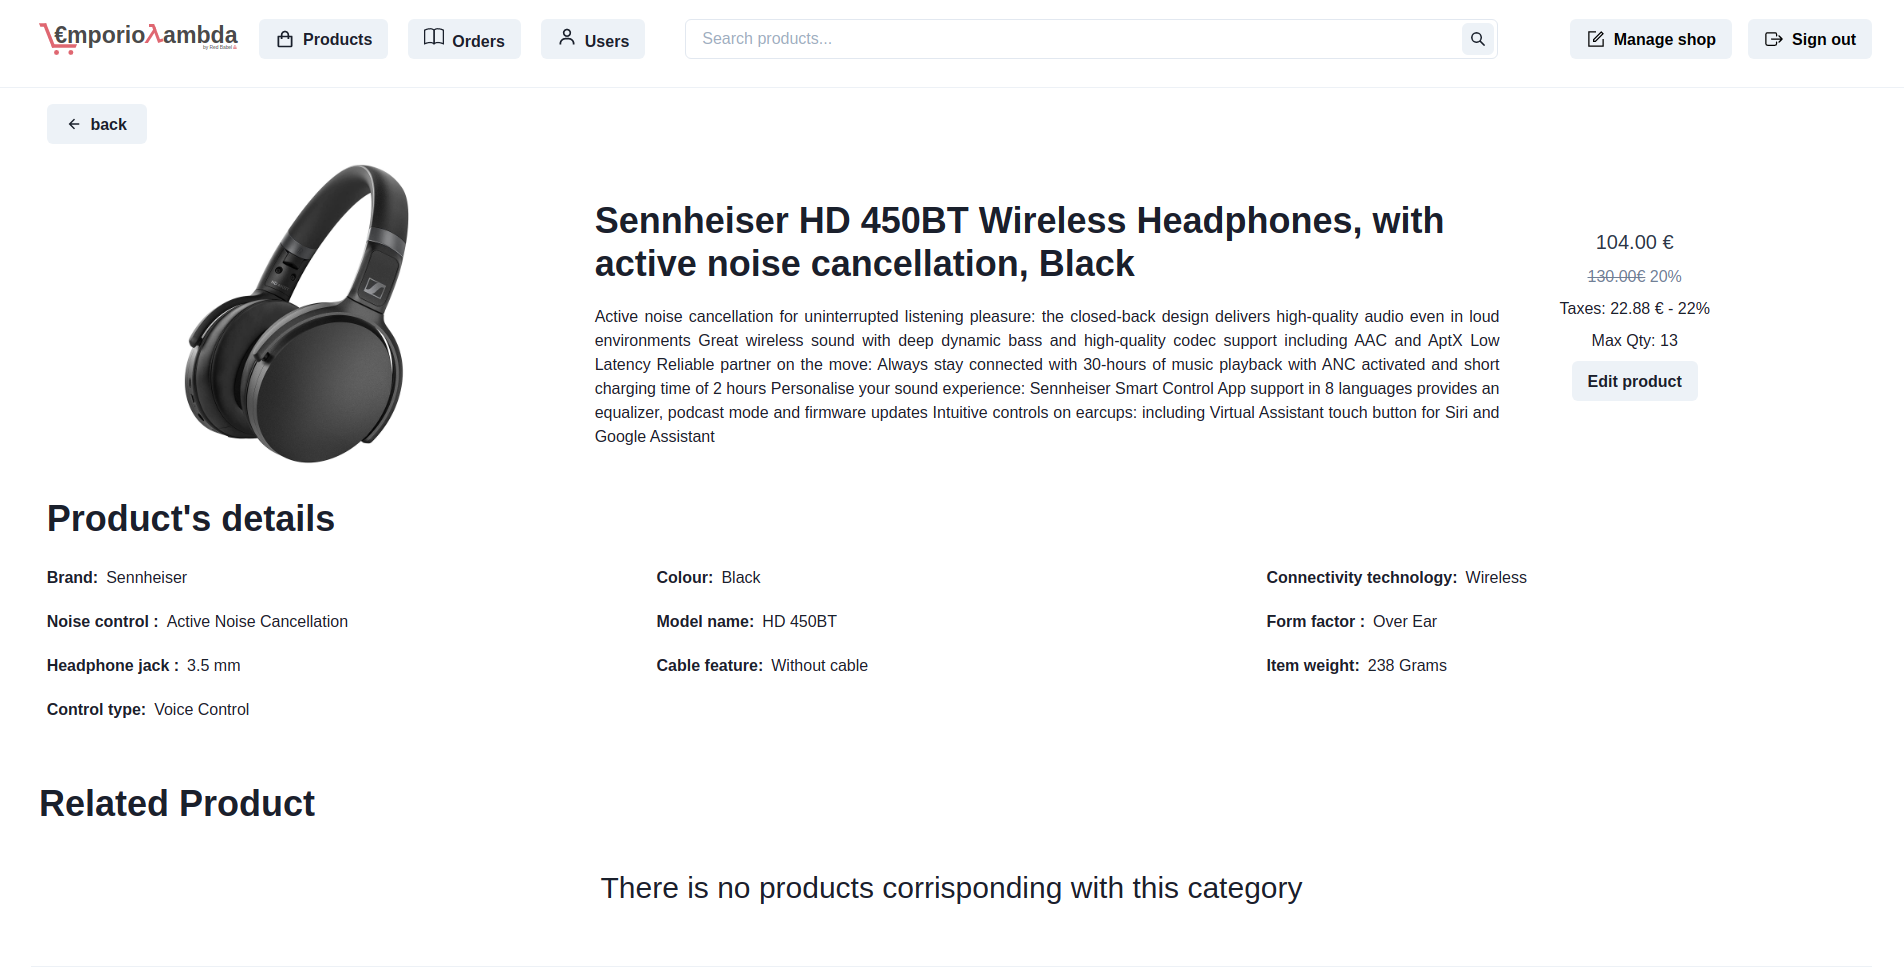
\includegraphics[scale=0.25]{../../../../Images/userManual/productDetailVendor.png}
    \centering
\end{figure}
\pagebreak
\subsubsection{Edit product}
By clicking on the \textit{Edit product} button on the right of the product detail screen, the vendor will be redirected to the screen where he can edit all the product details. After possibly changing the data, the vendor can save the changes by clicking on the \textit{Submit} button. From this screen it is also possible to delete the product by clicking on the \textit{DELETE PRODUCT} button.
\begin{figure}[!ht]
    \caption{Edit product page viewed from the vendor}
    \vspace{5px}
    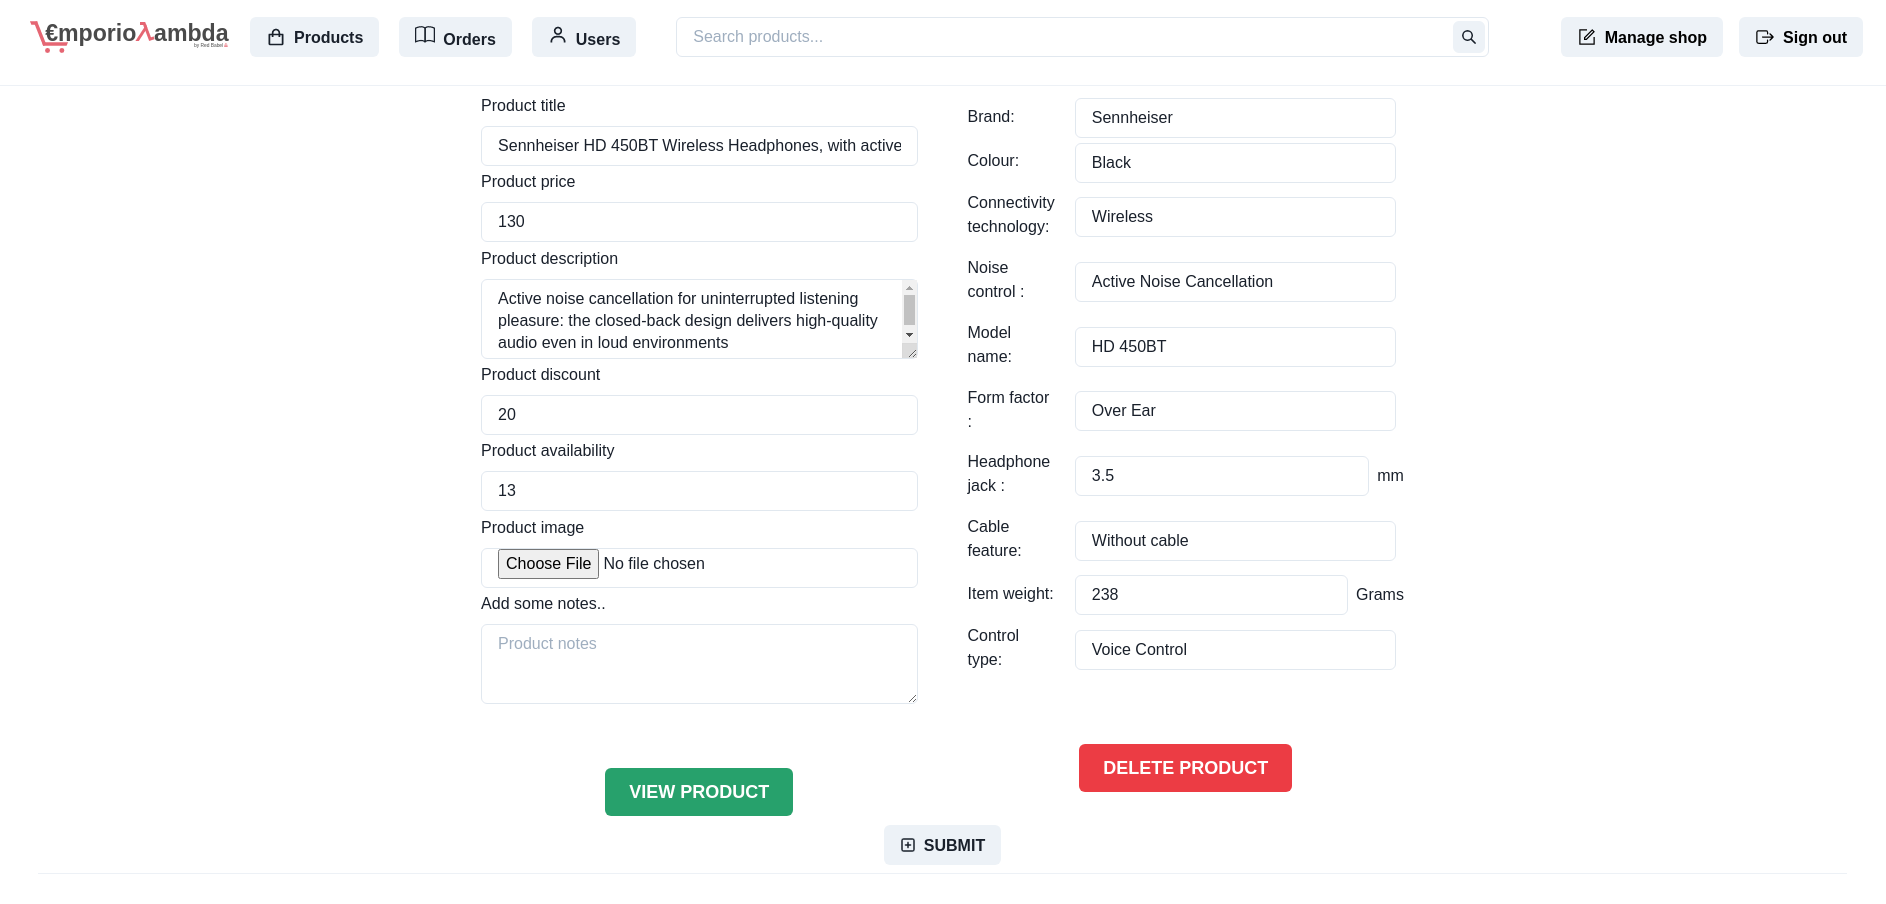
\includegraphics[scale=0.25]{../../../../Images/userManual/editProductVendor.png}
    \centering
\end{figure}

\section{Glossary}
\appendix
\subsection*{A}
\begin{itemize}
    \item \textit{Word} \\ definition
\end{itemize}
\section{}
\subsection*{Back-end} È la parte di codice di un programma che rappresenta la gestione dei contenuti e delle funzioni visibili nel Front-end.

\subsection*{BFF (Back-end For Front-end)} È uno strato tra l'user experience e le risorse che vengono utilizzate e punta a semplificare l'adattamento delle API alla UI.

\subsection*{Blockchain} È una struttura dati condivisa e immutabile. È un registro digitale in cui le voci sono raggruppate in blocchi concatenati in ordine cronologico; l'integrità è garantita dall'uso della crittografia.
\section{}
\begin{itemize}
    \item
\end{itemize}
\newpage
\section{}
\subsection*{D3.js} È una libreria JavaScript per creare visualizzazioni dinamiche ed interattive di pagine web.

\subsection*{Database} Sono un insieme di dati organizzati e strutturati,

\subsection*{Design pattern} È una soluzione progettuale generale ad un problema comune.

\subsection*{Driver} Sono porzioni di codiche che simulano chiamate all'unità in fase di test da parte degli utenti o del sistema.

\subsection*{DynamoDb} È un servizio database NoSQL proprietario, offerto da Amazon.

\subsection*{Diagrammi di Gant} È uno strumento di supporto alla gestione dei progetti.
\section{}
\newpage

\section{}
\subsection*{Framework} È un archittetura logica di supporto sulla quale un software può essere progettato e realizzato.
\subsection*{Frontend} Il forntend è la parte visiva dell'applicazione ossia la UI. Va gestire come gli utilizzatori della piattaforma andranno ad interagire con il backend ossia la parte amministrativa.
\section{}
\subsection*{Git}
È un sistema di controllo della versione distribuito per tenere traccia delle modifiche al codice sorgente durante lo sviluppo del software. Progettato per coordinare il lavoro tra i \textit{Programmatori}, ma utilizzabile per tenere traccia delle modifiche in qualsiasi set di file. I suoi obiettivi sono velocità, integrità dei dati e supporto per flussi di lavoro distribuiti e non lineari.

\subsection*{GitHub}
È un servizio di hosting per progetti software. È una implementazione dello strumento di controllo versione distribuito Git.

\subsection*{GitLab} È una piattaforma web open source che permette la gestione di repository Git e di funzioni trouble ticket.

\subsection*{gRPC} È un moderno sistema di \textit{remote procedure call} che, grazie a tecniche di processo innovative, rende possibile una comunicazione particolarmente efficiente all’interno delle architetture client-server distribuite.

\subsection*{GUI (Graphical User Interface)} È un tipo di interfaccia utente che consente l'interazione uomo macchina attraverso rappresentazioni grafiche.
\section{}
\begin{itemize}
    \item
\end{itemize}
\newpage
\section{}
\subsection*{IDE (Integrated Development Environment)} È un ambiente di sviluppo che aiuta i programmatori nella fase di sviluppo, debugging del codice sorgente di un programma.

\subsection*{IoT (Internet of Things)} Si riferisce all'estensione di Internet agli oggetti di tutti i giorni e ai luoghi.

\subsection*{ISO/IEC 12207:1995} È uno standard dell'ISO relativo alla gestione del ciclo di vita del software. Definisce tutte le attività svolte nel processo di svilippo e di mantenimento del software.

\subsection*{Issue}

\section{}
\begin{itemize}
    \item
\end{itemize}
\newpage
\section{}
\subsection*{Kafka} È una piattaforma open source di stream processing scritta in Java e Scala.. Il progetto mira a creare una piattaforma a bassa latenza ed alta velocità per la gestione di feed dati in tempo reale.

\subsection*{Kubernetes as a Service} È un servizio di autoamzione di \textit{Kubernetes}\textsubscript{\textbf{G}}, che fornisce delle API che si aggiornano ad ogni modifica dei componenti. Fornisce quindi dei servizi per un migliore sviluppo delle applicazioni basaste su Kubernets;

\subsection*{Kubernetes} Servizio open source per la gestione di applicazioni sviluppate attraverso containter. Progetto inizialmente sviluppato da Google, è ora open-source, I containter per mettono di testare l'applicazione in ambiti semireali andadno a simulare le concorenze e le esigenze dei sistemi reali.

\section{}
\subsection*{\LaTeX} È un linguaggio di markup per la preparazione di testi, basato sul programma di composizione tipografica TEX;
\section{}

% \subsection*{M2M (Machine to Machine)} È una tecnologia in grado di mettere in comunicazione diverse macchine tra loro, permettendo così lo scambio di dati ed informazioni acquisite al fine di migliorare i processi svolti dalle macchine stesse.

% \subsection*{Machine learning} È una branca dell'intelligenza artificiale. È un metodo di analisi di dati che automatizza la costruzione di modelli analitici. L'intervento umano è ridotto al minimo.

% \subsection*{Metodi di callback} Sono metodi che vengono passati ad altri metodi come parametri.

% \subsection*{Metodi ricorsivi} È un algoritmo la cui esecuzione su un insieme di dati comporta la semplificazione o suddivisione dell'insieme di dati e l'applicazione dello stesso agli insiemi di dati semplificati.

% \subsection*{Microservices architecture} È un architettura che suddivide un’applicazione in una serie di parti più piccole e specializzate, ciascuna delle quali comunica con le altre attraverso interfacce comuni come API e interfacce REST per creare un’applicazione.

% \subsection*{MIT} La Licenza MIT è una licenza di software libero creata dal Massachusetts Institute of Technology.

% \subsection*{Modello a V} un processo di sviluppo software che prevede lo sviluppo dei test in parallelo alle attività di analisi e progettazione.

% \subsection*{MQTT} È un protocollo ISO standard di messaggistica leggero di tipo \textit{publish-subscribe} posizionato in nel livello superiore di TCP/IP. È stato progettato per le situazioni in cui è richiesto un basso impatto e dove la banda è limitata. Il pattern \textit{publish-subscribe} richiede un message broker. Il broker è responsabile della distribuzione dei messaggi ai client destinatari.

% \subsection*{MVC (Model View Controller)} È un design architetturale orientato alla programmazione ad oggetti  e allo sviluppo di applicazioni web. Il suo punto forte è quello di avere una netta separazione tra parte logica e di business e la vista.
\subsection*{Microservices}
Microservices - also known as the microservice architecture - is an architectural style that structures an application as a collection of services that are
\begin{itemize}
    \item highly maintainable and testable;
    \item loosely coupled;
    \item independently deployable;
    \item organized around business capabilities;
    \item owned by a small team.
\end{itemize}
The microservice architecture enables the rapid, frequent and reliable delivery of large, complex applications. It also enables an organization to evolve its technology stack. 

\subsection*{N}
\begin{itemize}
    \item \textit{Navbar} \\ is a section of a graphical user interface intended to aid visitors in accessing information.
\end{itemize}
\section{}
\begin{itemize}
    \item
\end{itemize}
\newpage
\subsection*{P}
\begin{itemize}
    \item \textit{Word} \\ definition
\end{itemize}
\subsection*{Q}
\begin{itemize}
    \item \textit{Word} \\ definition
\end{itemize}
\section{}
\subsection*{React} È una libreria JavaScript per la creazione di interfacce utente, è specifico per la creazione di applicazioni mobile.

\subsection*{Responsabile di Progetto} Il Responsabile di progetto è una figura importante per la gestione di progetto in quanto ricadono su di lui le responsabilità di pianificazione, gestione, controllo e coordinamento. Un altro suo compito è quello di fare da intermediario nella comunicazione tra il gruppo e i soggetti esterni: sono quindi di sua competenza le comunicazioni con committente e proponente.

\subsection*{RFID} È una tecnologia per l'identificazione e/o memorizzazione automatica di informazioni inerenti a oggetti, animali o persone  basata sulla capacità di memorizzazione di dati da parte di particolari etichette elettroniche, chiamate tag , e sulla capacità di queste di rispondere all'interrogazione a distanza da parte di appositi apparati fissi o portatili, chiamati reader.
\newpage
\section{}
\begin{itemize}
    \item
\end{itemize}
\newpage
\section{}
\subsection*{Technology Baseline} Definisce le tecnologie, i framework e i servizi scelti per la realizzazione del prodotto.

\subsection*{Test end-to-end} È una metodologia utilizzata per verificare se il flusso di un'applicazione si sta comportando come progettato dall'inizio alla fine senza che vengano rilevati dei \textit{failure} che andrebbero a inficiare sulla qualità dell'applicazione stessa.

\subsection*{Ticketing} È un sistema che permette di comunicare segnalazioni o problemi all'interno di GitHub.

\subsection*{Tomcat} È un server web open source. Implementa le specifiche \textit{JavaServer Pages} e \textit{servlet}, fornendo quindi una piattaforma software per l'esecuzione di applicazioni web sviluppate in linguaggio Java.

\subsection*{TypeScript} Si tratta di un Super-set di JavaScript. Il linguaggio estende la sintassi di JavaScript in modo che qualunque programma scritto in JavaScript sia anche in grado di funzionare con TypeScript senza nessuna modifica. È stato progettato per lo sviluppo di grandi applicazioni ed è destinato a essere compilato in JavaScript per poter essere interpretato da qualunque web browser o app.
\section{}
\subsection*{UI (User Interface)} È l'intefaccia uomo-macchina che permette all'utente di interagire con la macchina.

\subsection*{UML} È un linguaggio di modellazione e di specifica basato sul paradigma ad oggetti. Viene utilizzati per relizzazione di vari diagrammi:
\begin{itemize}
    \item diagramma delle classi;
    \item diagramma di attività;
    \item diagramma sequenza;
    \item diagramma dei casi d'uso.
\end{itemize}
\section{}
\subsection*{Verificatore} Il Verificatore si occupa di controllare il prodotto del lavoro svolto dagli altri membri del gruppo, sia esso codice o documentazione. Per le correzioni si affida agli standard definiti nelle Norme di Progetto.

\subsection*{Visual Studio Code} È un editor di codice sorgente nclude il supporto per debugging, un controllo per Git integrato, Syntax highlighting, IntelliSense, Snippet e refactoring del codice.
\newpage
\section{}
\begin{itemize}
    \item
\end{itemize}
\newpage
\section{}
\begin{itemize}
    \item 
\end{itemize}
\newpage
\section{}
\begin{itemize}
    \item 
\end{itemize}
\newpage
\section{}
\begin{itemize}
    \item
\end{itemize}
\newpage

\end{document}


